\documentclass[11pt]{article}
\usepackage{mypackage}

\begin{document}

{\fontfamily{cmr}\selectfont
\title{ \normalsize \textsc{}
		\\ [2.0cm]
		\HRule{0.5pt} \\
		\LARGE \textbf{\uppercase{Parameter Study on Aeroelastic Response of  High Aspect-Ratio Wings}
		\HRule{2pt} \\ [0.5cm]
		\normalsize \today \vspace*{5\baselineskip}}
		}
}

\date{}

\author{
        \textit{Student}: Dharapa Pattanakul\\ 
        \textit{Supervisor}: Branislav Titurus\\
		University of Bristol \\
		Department of Aerospace Engineering }

\vfill
\titlepic{\includesvg[width = .3\textwidth]{figures/Hpic.svg}}
\maketitle
\thispagestyle{empty}
%\cleardoublepage


%%%%%%%%%% Executive Summary %%%%%%%%%
\newpage
\pagenumbering{roman} 
%\thispagestyle{empty}
\section*{Executive Summary}
%\begin{itemize}
%    \item use a nice graph
%    \item simplified and annotated
%\end{itemize}
This study was carried out to develop a computational model for a parameter study on aeroelastic responses in an aircraft with high aspect ratio (AR) wings. High AR wings are being looked at as an alternative to a current configuration of commercial aircraft as this new design is more environmental friendly: provides a higher lift-to-drag ratio and longer ranges. However, the increase in structural flexibility of the wing makes this configuration more prone to catastrophic aeroelastic responses.\\

\textbf{Section \ref{sec:prob-def}} defines the problems that arise in the existing method of analysing aeroelastic behaviour of the high AR wing: the computational model does not provide a sufficiently accurate result in most cases when compared to flight-test data. Furthermore, the improved high fidelity models are usually too time consuming and too expensive to be widely adapted.\cite{Jones2015PreliminaryExperiment}\\

Background theories used in this study were outlined in \textbf{Section \ref{sec:background}} where the inertia model (no coupling between modes), aerodynamic model (unsteady aerodynamics) and structural model (two assumed shapes) were explained. These models were combined for the analysis of flutter and divergence behaviour. Section \ref{sec:lit-rev} presents the findings from literature review. The information and background researches were essential for this project to satisfy the aim and objectives listed in \textbf{Section \ref{sec:aim+obj}} with the main aim being the development of a computational model for aeroelastic behaviour analysis for high AR wings. \\

\textbf{Section \ref{sec:method}} explains the approach and steps taken to yield the results from the parameter study. The eigenvalue solution method was briefly explained as a way to obtain the flutter speed and divergence speed. Comparisons against existing experimental/analytical results was the approach taken to validate the model. The errors and discrepancies resulting from the lack of nonlinearlities in the model were quantitatively illustrated in table \ref{tab:error}.\\

The results from the preliminary studies including the initial conclusions were presented in \textbf{Section \ref{sec:prelim}}. Figure \ref{fig:exec-flutt} shows the flutter speed calculation for the NASA's SUGAR High conceptual design model (a high AR wing aircraft) and figure \ref{fig:exec-div} shows divergence speeds. 

\begin{figure}[!hbt]
    \begin{minipage}{.5\textwidth}
    \centering
    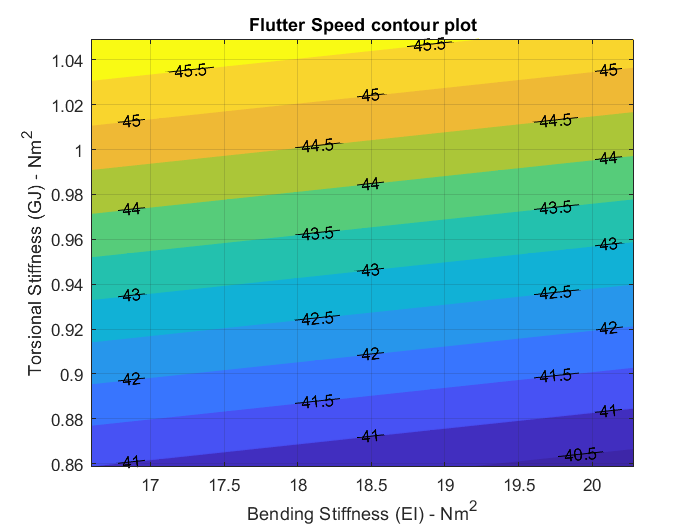
\includegraphics[width = \textwidth]{figures/flutter.png}
    \caption{SUGAR High flutter plot}
    \label{fig:exec-flutt}
    \end{minipage}%
    \begin{minipage}{.5\textwidth}
    \centering
    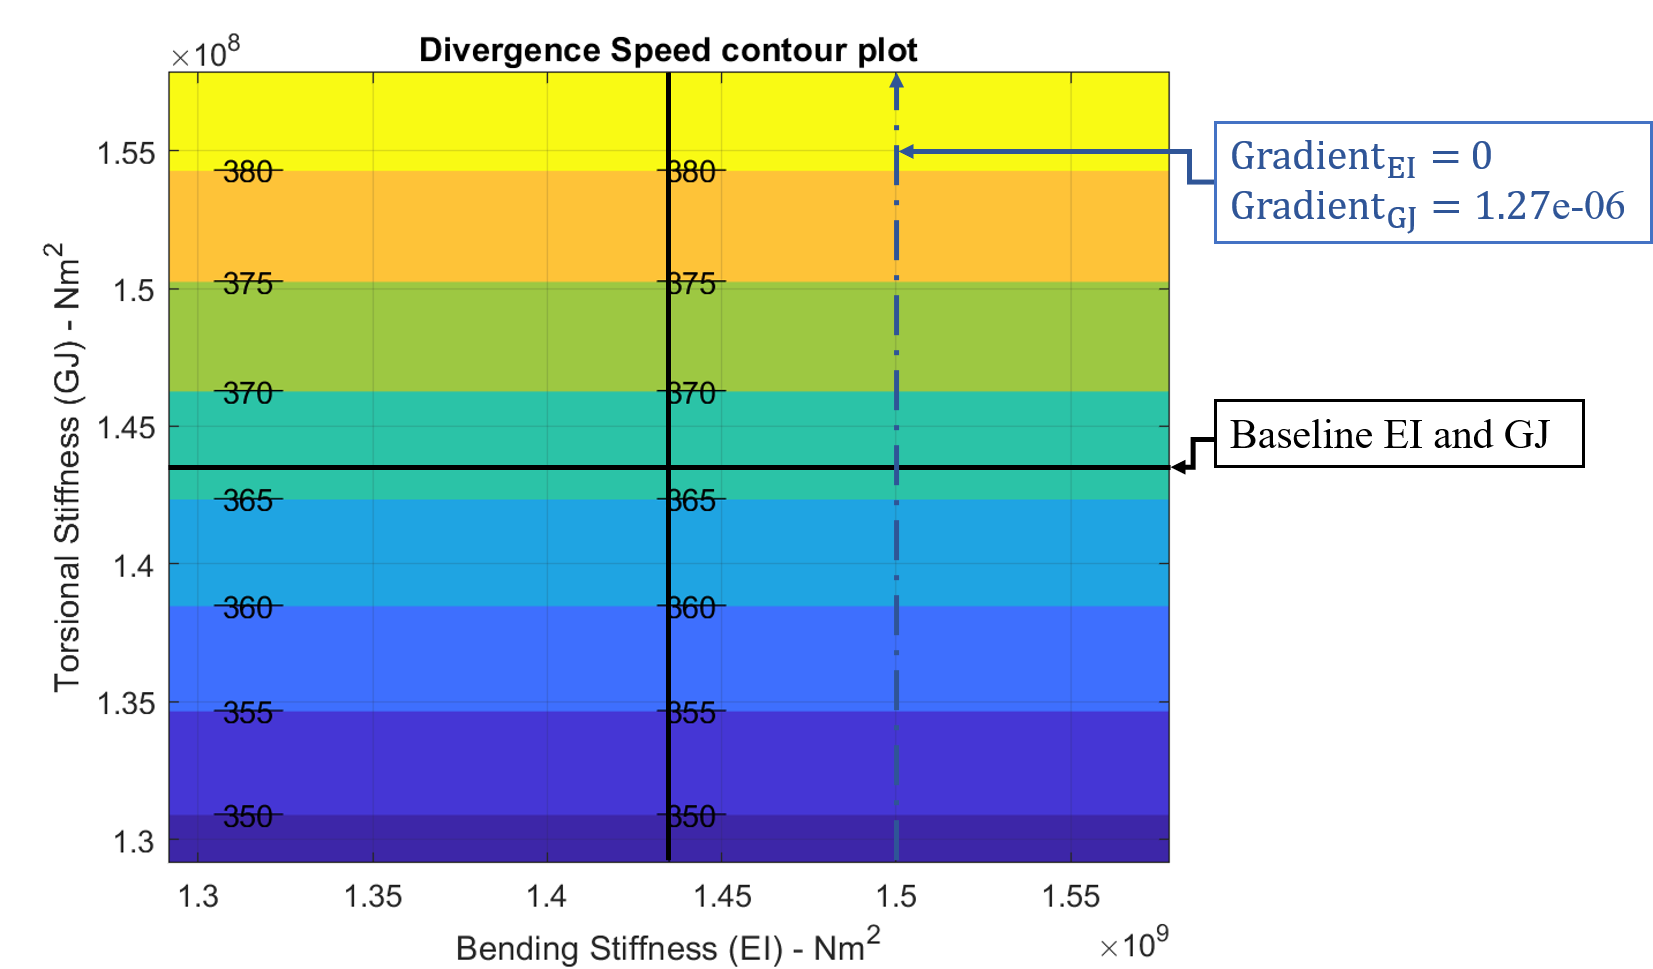
\includegraphics[width = \textwidth]{figures/divergence.png}
    \caption{SUGAR High divergence plot}
    \label{fig:exec-div}
    \end{minipage}
\end{figure}
Both of these figures show how flutter speed and divergence speed changes with varying bending stiffness (EI) and torsional stiffness (GJ). It can be concluded that both EI and GJ affect flutter speed but EI has a bigger impact. While for divergence, EI has no effect and GJ has a big impact.\\

Finally, the risks in this project and the ways to mitigate them were explained in \textbf{Section \ref{sec:risk}}. The main risks include the risk of not being able to produce a workable model and the risk of not being able to obtain usable parameters. They were mitigated by sectioning a sufficient amount of time for both research and code development. The improvement for future work on the model was described in \textbf{Section \ref{sec:future-work}}. This includes further development to cater for nonlinearities and the inclusion of Limit Cycle Oscillation analysis. 
\cleardoublepage

%----------- table of contents ----------%
\newpage
\tableofcontents
%\thispagestyle{empty}
\newpage
\listoffigures
%\thispagestyle{empty}
\addcontentsline{toc}{section}{\numberline\ {}List of figures}
%\cleardoublepage
%List of tables 
\listoftables
%\thispagestyle{empty}
\addcontentsline{toc}{section}{\numberline\ {}List of tables}
%\cleardoublepage
%\newpage

\section*{Nomenclatures}
\begin{table}[H]
    %\centering
    %\caption{Wing model parameters}
    \includestandalone{tables/nomen}
    \label{tab:nomen}
\end{table}
\cleardoublepage
%----------------------------------------%
\pagenumbering{arabic} 
%%%%%%%%%% Problem Definition %%%%%%%%%%
\newpage
\section{Problem Definition}
\label{sec:prob-def}
%\begin{itemize}
%   \item Parameters study on High AR wings to observe flutter and divergence
%   \item The need for High AR - environmentally friendly
%   \item widely study as a linear system and there are some literature
%   \item Not enough nonlinear study
%   \item Not enough parameter study
%   \item Results
%   \item Results
%   \item Results
%\end{itemize}
%\subsection{Scope} 
There is a strive for greener innovations that can be seen across the aviation industry. These ideas attempt to maximise flight efficiency while minimises environmental impact. One way to achieve this is by increasing wings' aspect-ratio (AR). This provides a higher lift-to-drag ratio and a longer range. However, this configuration has not yet been widely adapted into commercial jets due to a few limiting factor such as limiting spaces in airports. One of the important limiting factor is the flexibility of high AR wings; large deformation results in aeroelastic behaviour.\\ 

The advantages given above has attracted many attention to the study of aeroelasticity for high AR wing configurations. Several computational and experimental study have been done on the aeroelastic responses of unmanned aerial vehicles (UAV) over the past few decades, but only a few on commercial aircraft. This project will seek to develop a computational model for aeroelastic study for high AR wings. The nonlinear method was chosen for the better understanding of the coupling between structural deformation and aeroelastic response.\\

In this project, the parameter study was carried out to improve the understanding of how each properties affect the aeroelastic behaviour. This is useful for future design of the aircraft of high AR configuration or the purpose of aeroelastic tailoring. The main challenge faced in this project was the lack of studies to be used as a baseline. The main requirement of existing literature is that the study was done and deemed suitable for high AR wings.

%%%%%%%%%% Background %%%%%%%%%%
\section{Background}
\label{sec:background}
\iffalse
\begin{itemize}
    \item Aeroelasticity - Cooper
    \begin{itemize}
        \item Structure
        \item Aerodynamics
        \item Inertia
    \end{itemize}
    \item Flutter - mohemmed
    \item Divergence
    \item High AR and nonlinearities
    \item Model development (1p)
    \item Parameters acquisition (1/2p)
\end{itemize}
\fi
\subsection{Aeroelasticity}
Aeroelastic phenomena occurs when there is an interaction between structures and aerodynamics force in a model. This is predominant in a structure of high flexibility such as a high aspect-ratio (AR) wing. This means the aircraft with such property are more sensitive to flutter and divergence. Failure to predict the occurrence of these phenomenons can results in an aircraft losing its control, failing air worthiness regulations and a fatal structural damage.\\

%------ wrapped figure of triangle -----
\begin{wrapfigure}{r}{8.5cm}
    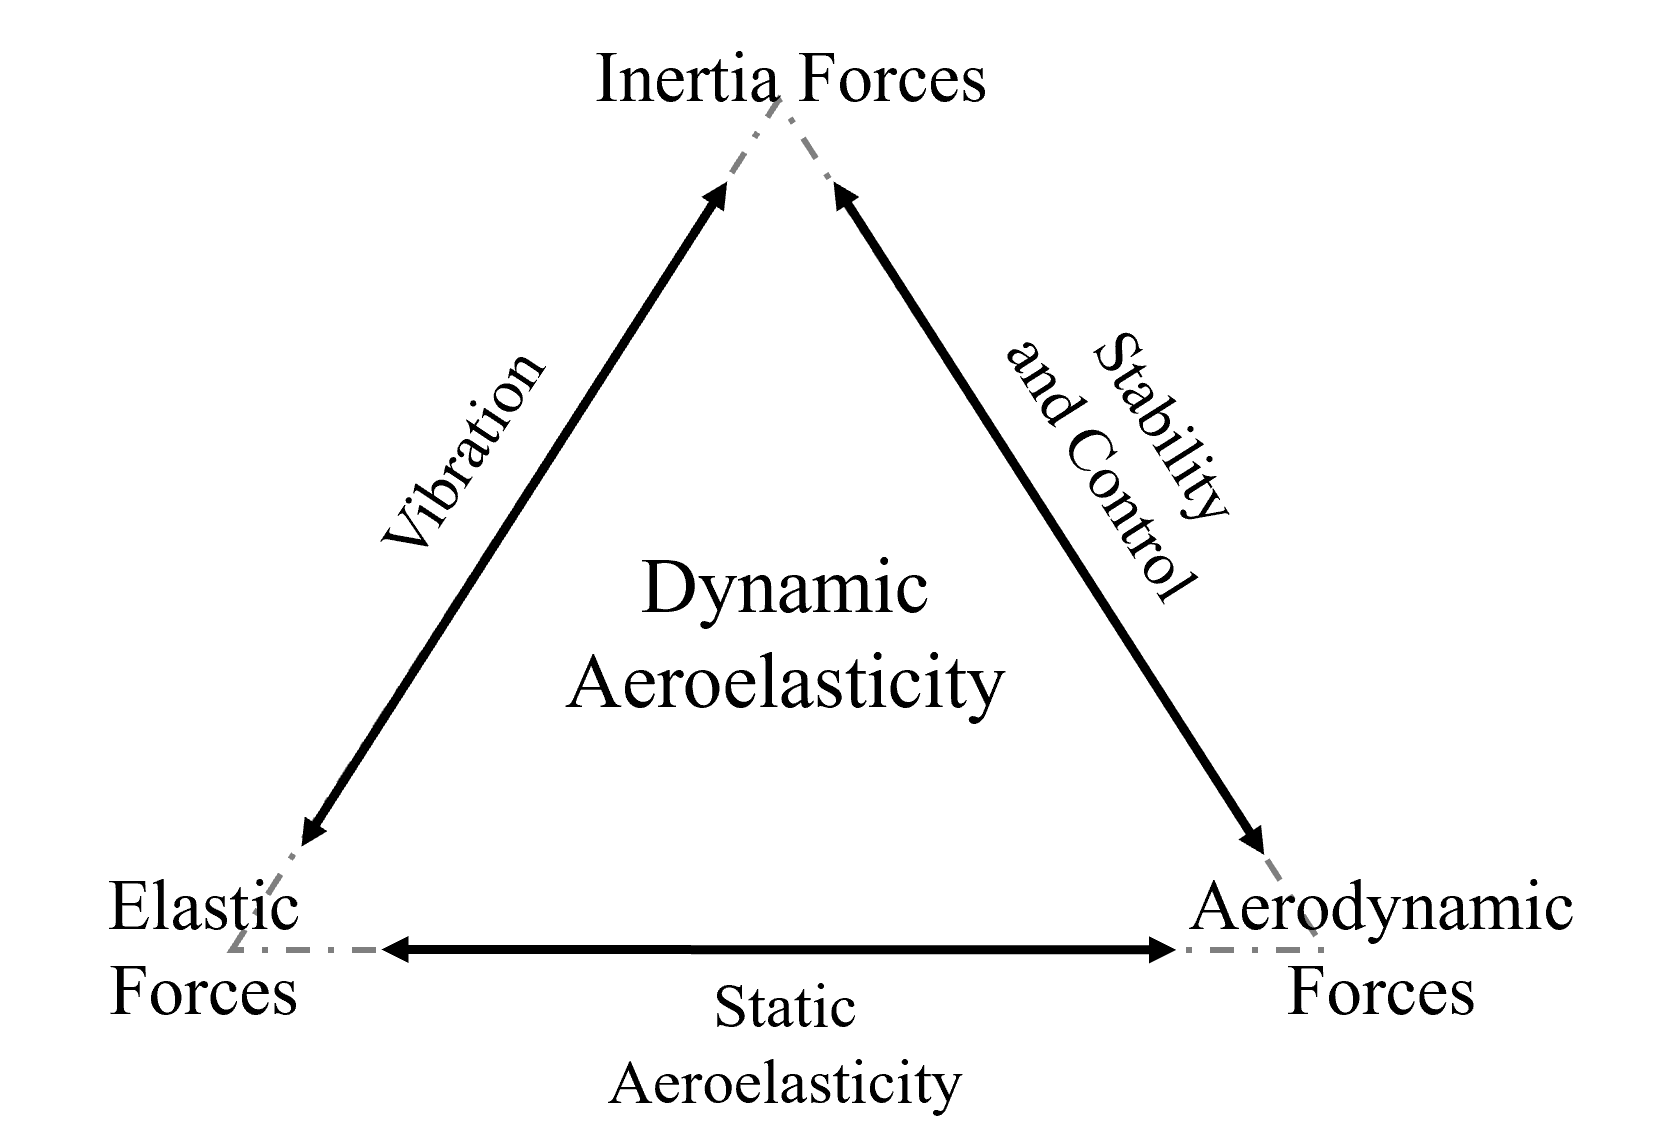
\includegraphics[width=8.5cm]{figures/aerotri.png}
    \caption{Aeroelastic triangle}
    \label{fig:aero-tri}
\end{wrapfigure} 
%----------------------------------------

This study will investigate the affects of torsional stiffness and bending stiffness on flutter and divergence in a high AR wing. The study involves the three main forces that contribute to aeroelasticity: aerodynamic, elastic and inertia (as shown in figure \ref{fig:aero-tri}).\\

Each component and the assumptions in the model which make up the aeroelastic phenomena are explained in section \ref{sec:inertia} - \ref{sec:struc}. The Aeroelastic phenomena are explained in section \ref{sec:aero-phe}. The responses considered here include both dynamic and static aeroelasticity. Dynamic response involves a study of flutter behaviour which disturbs aircraft stability and is influenced by oscillations of the structure. While static response focuses on the deformation of the structure and its effect of lift distribution.
\newpage
\subsubsection{Inertia}
\label{sec:inertia}
The inertia matrix can be represented as 
\begin{gather*}
    \begin{bmatrix}A_{bb} & A_{bt} \\ A_{tb} & A_{tt} \end{bmatrix}
\end{gather*}
Where $b$ repreesnts bending terms and $t$ represents torsion terms. However, as there is no inertia coupling in the model, $A_{bt} = A_{tb} = 0$. This allows the bending stiffness ($EI$) and the torsional stiffness ($GJ$) to be represented in term of the torsion and bending natural frequencies as
\begin{equation}
    \omega_b = \sqrt{\frac{4EI}{A_{bb}s^3}} \text{ and } \omega_t = \sqrt{\frac{GJ}{A_{tt}s}}
\end{equation}

\subsubsection{Aerodynamics}
The aerodynamic model implemented here is a strip theory aerodynamics with additional simplified unsteady aerodynamic terms. This model includes the frequency dependent effect on lift and pitching moment which is essential for flutter analysis. The simplified expressions for lift increments ($dL$) and nose up pitching moment ($dM$) as a result of generalised unsteady aerodynamic forces applied with the strip theory are 
\begin{align}
dL &= \frac{1}{2}\rho V^2ca_w\Big( \frac{y^2\dot{q_1}}{s^2V}+\frac{y}{s}q_2\Big)dy\\
dM &= \frac{1}{2}\rho V^2 c^2\Big[ea_w\Big(\frac{y^2\dot{q_1}}{s^2V}+\frac{y}{s}q_2\Big)+M_{\dot{\theta}}c\frac{(y\dot{q_2})}{4sV}\Big]dy
%\label{eq:unsteady-aero-moment}
\end{align}
\iffalse
\begin{align}
L &= \rho V^2 \Big{(}L_z z + L_{\dot z}\frac{b\dot z}{V}+L_{\theta}b\theta + L_{\dot \theta}\frac{b^2 \dot \theta}{V}\Big{)} \\
M &= \rho V^2 \Big{(} M_z bz + M_{\dot z} \frac{b^2 \dot z}{V} + M_{\theta} b^2 \theta + M_{\dot \theta} \frac{b^3 \dot \theta}{V} \Big{)}
\end{align}
\fi

\begin{wrapfigure}{l}{9cm}
    \centering
    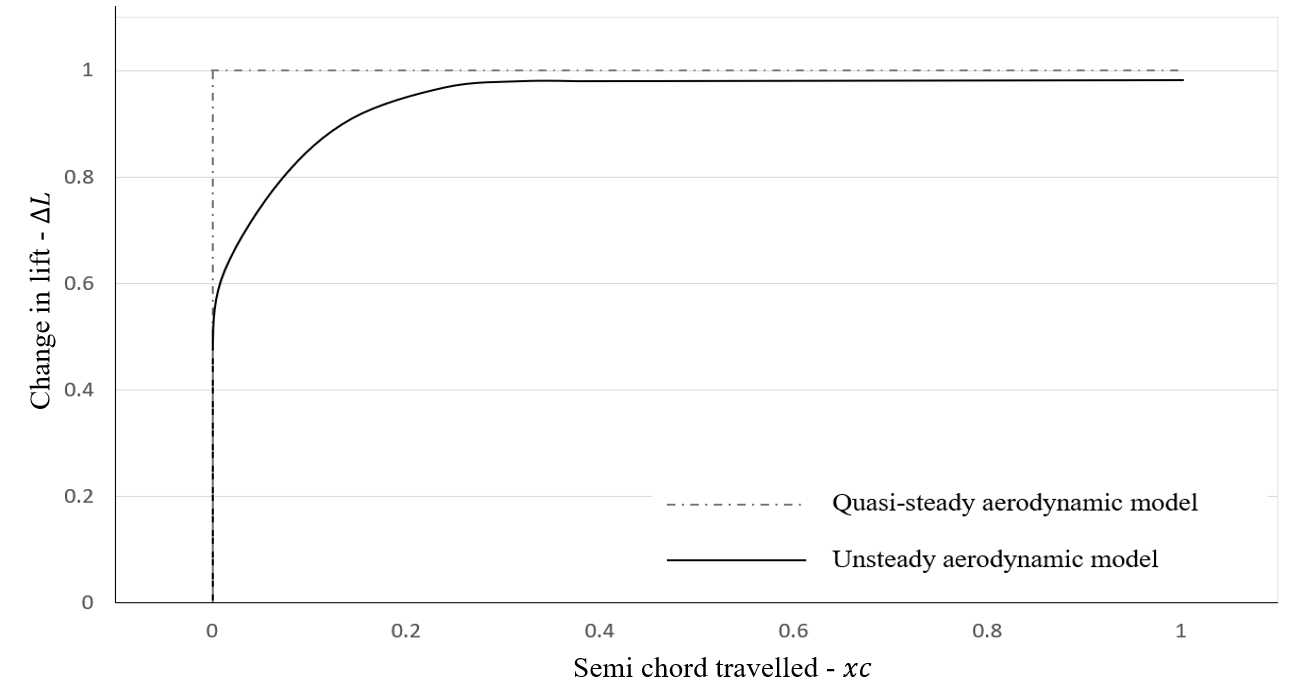
\includegraphics[width = 9cm]{figures/wagner-func.png}
    \caption{Change in lift due to change in angle of incidence.}
    \label{fig:wagner}
\end{wrapfigure}

The change in lift due to a change in angle of incidence as modelled using an unsteady aerodynamic model can be illustrated by the Wagner Function (figure \ref{fig:wagner}). The function shows that lift takes time to build up as the  airflow travels across the semi-chord of the lifting surface. The quasi-steady model assumes a sharp step change in lift as it does not include time-effect; assumes instantaneous. This can results in a substantial aeroelastic modelling errors \cite{Wright2015INTRODUCTIONLOADS}. The pitch damping term $M_{\dot{\theta}}$ is included in equation (2) to include the time delay effect. This property is negative and will be treated as a constant in this model.\\ \\
\iffalse
\begin{figure}[H]
    \centering
    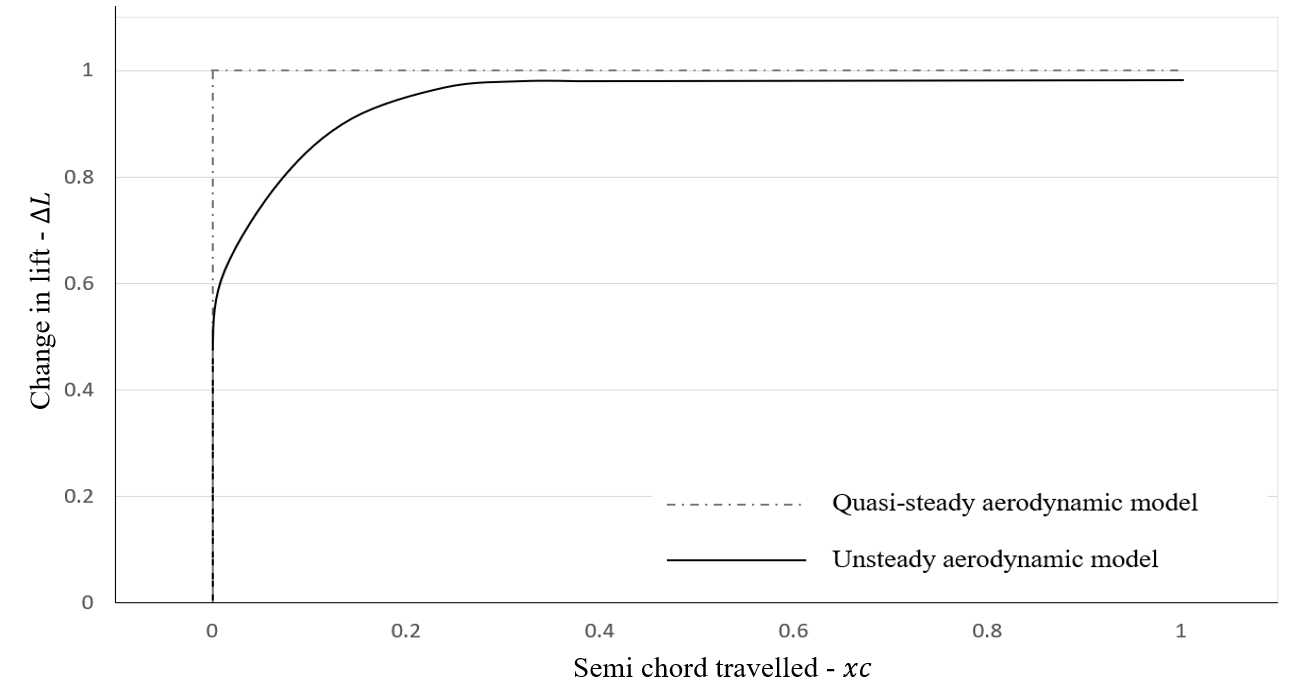
\includegraphics[width = .7\textwidth]{figures/wagner-func.png}
    \caption{Change in lift due to change in angle of incidence.}
    \label{fig:wagner}
\end{figure}
\fi

\subsubsection{Structure}
\label{sec:struc}
The structural model used in this analysis is the binary wing aeroelastic model. This implies that the wing is a flexible rectangular, unswept, cantilever wing with one bending and one torsion assumed shape \\
\iffalse
(as shown in figure \ref{fig:free-free}).
\begin{figure}[H]
    \centering
    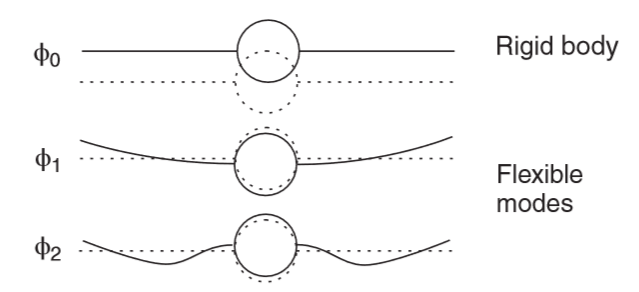
\includegraphics[width = .6\textwidth]{figures/free-free-mode-shape.png}
    \caption{Full aircraft 'Free-Free' assumed mode shapes}
    \label{fig:free-free}
\end{figure}
\fi
The kinetic energy ($T$) due to the dynamic motion and the elastic potential energy ($U$) corresponding to the strain energy in bending and torsion can be written as
\begin{align}
    T &= \frac{m}{2}\int_0^s \int_0^c \Big( \Big{(} \frac{y}{s}\Big{)}^2\dot{q_1}+\Big{(}\frac{y}{s}\Big{)}(x-x_f)\dot{q_2}\Big{)}^2dxdy\\
    U &= \frac{1}{2}\int_0^s EI \Big{(}\frac{2q_1}{s^2}\Big{)}^2dy+\frac{1}{2}\int_0^sGJ\Big{(}\frac{q_2}{s}\Big{)}^2dy
\end{align}

Where $q_1$ and $q_2$ are generalised coordinates corresponding to the simple assumed shapes in bending and torsion consecutively. Uniformed distribution of mass is assumed here. 


\subsection{Aeroelastic phenomena}
\label{sec:aero-phe}
%Aeroelastic phenomena can be categorised into two categories: \textbf{dynamic} and \textbf{static}.  

\iffalse
\begin{figure}[H]
    \centering
    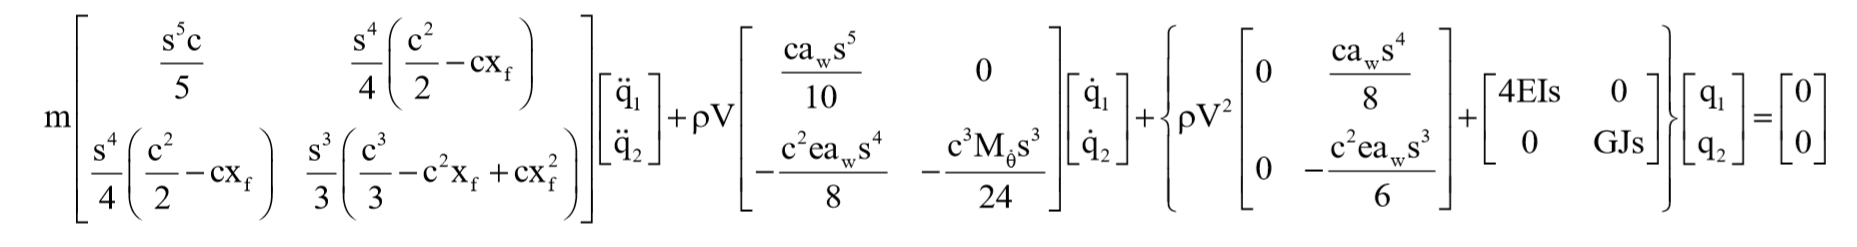
\includegraphics[width=\textwidth]{figures/EQ.png}
    %\caption{Full Aeroelastic Equation}
    \label{fig:aero-eq}
\end{figure}
\fi

%\textbf{Apply Lagrange to get this - just mention it briefly - simple form is enough - REFERENCE THE BOOK!}

\begin{equation}\label{eq:full-aeroe}
\begin{gathered}
\begin{split}
    m\begin{bmatrix} \frac{s^5c}{5} & \frac{s^4}{4}\Big{(}\frac{c^2}{2}-cx_f\Big{)} \\ \frac{s^4}{4}\Big{(}\frac{c^2}{2}-cx_f\Big{)} & \frac{s^3}{3}\Big{(}\frac{c^3}{3}-c^2x_f+cx_f^2\Big{)} \end{bmatrix} \begin{bmatrix}\ddot{q_1}\\ \ddot{q_2} \end{bmatrix} + \rho V \begin{bmatrix} \frac{ca_w s^5}{10} & 0 \\ -\frac{c^2e a_w s^4}{8} & -\frac{c^3M_{\dot\theta}s^3}{24} \end{bmatrix}\begin{bmatrix}\dot{q_1}\\ \dot{q_2}\end{bmatrix} +\\ \Bigg{\{}\rho V^2  \begin{bmatrix} 0 & \frac{ca_ws^4}{8} \\ 0 & -\frac{c^2ea_ws^3}{6} \end{bmatrix} + \begin{bmatrix} 4EIs & 0 \\ 0 & GJs \end{bmatrix} \Bigg{\}}\begin{bmatrix} q_1 \\ q_2 \end{bmatrix} = \begin{bmatrix} 0 \\ 0 \end{bmatrix}
\end{split}
\end{gathered}
\end{equation}

Equation 6 is the main equation used in this study. It is obtained by applying Lagrange to the inertia, aerodynamic and structural terms described earlier.

%Static  aeroelastic  phenomena involves  the  study  of  the  deformation  of  the  aircraft  and  how  this influences  the  distribution  of  lift.  This  con sequently  causes  torsional  divergence  reducing  the effectiveness of the control surface. Static aeroelasticity is also no affected by mass properties of the  aircraft  and  is  not  influenced  by  oscillations.  Dynamic  aeroelastic  phenomena  involves the analysis of  flutter of the  aircraft which disturbs the stability of the aircraft and the air stream is subjected to extraction of energy from the aircraft structure. 

\subsubsection{Flutter}
Flutter is the most important dynamic flutter phenomena \cite{MohammedFREEWINGS}. It occurs when an aircraft loses its stability due to an extraction of energy from the air stream by the aircraft structure. Resulting in an oscillatory motion that does not decay and increases in magnitude over time. This phenomenon is undesirable as it damages the aircraft structure and wear out its life cycle.\\

Flutter boundary is defined as  the lowest speed at which a small perturbation to a static equilibrium results in flutter. Lowest airspeed at which the system has a complex conjugate pair of eigenvalues with zero real part. 
\vspace{-1cm}
\begin{figure}[H]
    \centering
    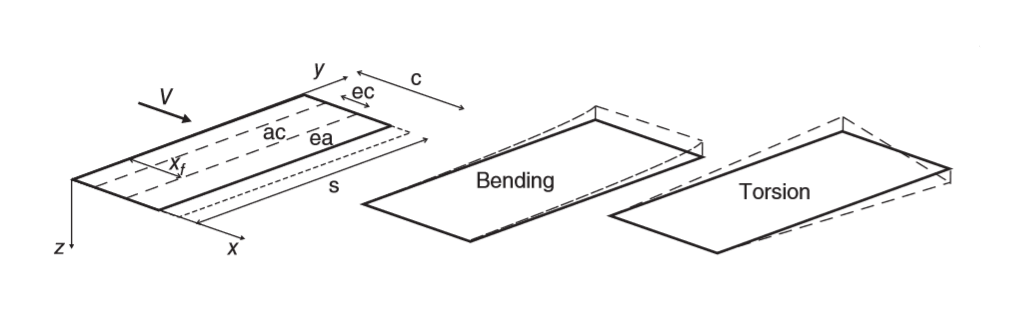
\includegraphics[width = .8\textwidth]{figures/torsion-bending-modes.png}
    \caption{Assumed mode shapes in torsion and bending mode.}
    \label{fig:binary}
\end{figure}

\subsubsection{Divergence}
Divergence is a static instability of a lifting surface of an aircraft. When the wing exceeds its torsional divergence speed, the torsional moment from aerodynamic force due to twist overcomes the structural elastic restoring moment. This causes the wing to become statically unstable\cite{RaymondL.Bisplinghoff2002PrinciplesAeroelasticity}. As the time-dependent can be neglected in the case of static phenomena, the inertia force can be neglected. \\
%------ wrapped figure of heave and pitch -----
\begin{wrapfigure}{l}{8.5cm}
    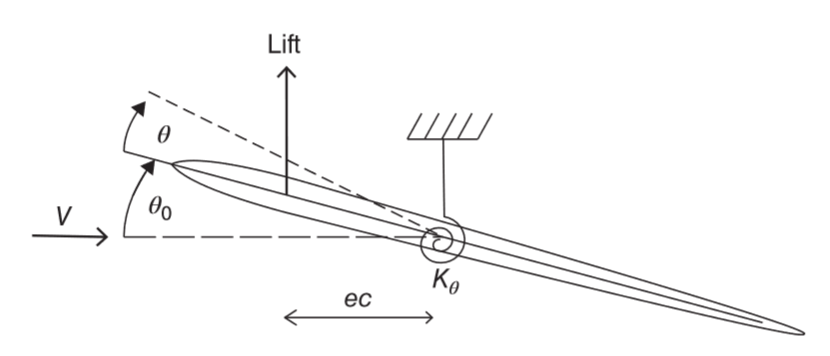
\includegraphics[width=8.5cm]{figures/two-dimensional-wing-torsional-spring.png}
    \caption{2D wing with a torsional spring.}
    \label{fig:torsional-spring}
\end{wrapfigure} 
%----------------------------------------
In a wing that is not stiff enough, divergence will cause the wing to twist off \cite{2011AeroelasticityFlutter}. Stiffness is much more important that strength in this case. In modern aircraft, flutter speed is usually lower than divergence speed; flutter usually occurs before divergence. However, this does not render divergence speed analysis to be obsolete as it is a good indication of the general stiffness of the aircraft structure and must be considered as part of the certification process \cite{Wright2015INTRODUCTIONLOADS}.\\ \\

\iffalse
Figure \ref{fig:torsional-spring} illustrates the torsional elastic moment($M_E$) versus the aerodynamic moment($M_{ac}$) and moment due to lift($ec.L$). Each term in the equilibrium can be expressed as:
\begin{eqnarray*}
ec.L = ec.qSC_{L,{\theta _0}}(\theta _0 + \theta),\hspace{1cm} M_{ac} = qScC_{M_{ac}},\hspace{1cm} M_E = K_{\theta}\theta
\end{eqnarray*}

%\begin{align*}
%\text{Lift:}\hspace{2cm} L &= qSC_{L,{\theta _0}}(\theta _0 + \theta)\\
%\text{Aero moment:}\hspace{1.6cm}M_{ac} &= qScC_{M_{ac}}\\
%\text{Elastic moment:}\hspace{1.65cm}M_E &= K_{\theta}\theta
%\end{align*}

\begin{equation}
qScC_{M_{ac}} + ec. qSC_{L,{\theta _0}}(\theta _0 + \theta) = K_{\theta}\theta
\end{equation}
\fi
\newpage
\subsection{High AR Wing}
\label{sec:high-AR}
\begin{wrapfigure}{r}{8.5cm}
    \centering
    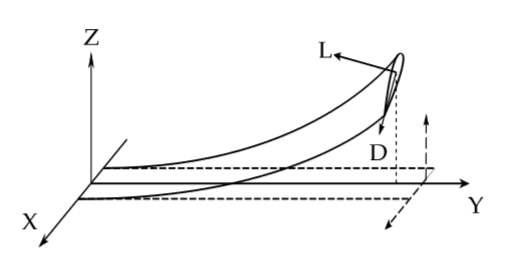
\includegraphics[width = 8.5cm]{figures/Eaton-highly-flexible-wing.png}
    \caption{Nonlinear loading on a high AR wing.}
    \label{fig:high-AR-load}
\end{wrapfigure}
High AR wings are the focused of this study as reasons mentioned in section \ref{sec:prob-def}. However, they are more flexible and more complicate to modelled. The increase in flexibility means a large elastic deformation is due to happen as the aircraft travels at higher speed. The need to understand aeroelastic phenomena in a high AR wing aircraft travelling near the transonic region was mentioned by Afonso et al \cite{Afonso2017AWings} for future development of high AR wing commercial jets.\\

 The complications surrounding the model can be deduced to be a result of nonlinearities in aerodynamic model. As the wing deflects upwards, the lift nolonger acts vertically to the lifting surface. This model is hard to mathematically described and with the limitations of time and resources for this project, the simplified model was adopted. With the nonlinear model being the aim for future development of the model.
%\textbf{TALK ABOUT THE IMPORTANCE ON HIGH AR + COMPLICATIONS SURROUNDING THE MODEL}

%%%%%%%%%%%%%%%%%%%%%%% LITERATURE REVIEW %%%%%%%%%%%%%%%%%%%%%%%
\subsection{Literature Review}
\label{sec:lit-rev}
Afonso et al\cite{Afonso2017AWings} reviewed the importance of nonlinear model in aeroelasticity. The need for more computational and experimental study was mentioned as the existing reduced order model gets more complicte as nonlinearity inceases. The lack of information concerning values for modal amplitudes in simulations was also recognised.\\

The linear model used in this project was based on Jan R. Wright and Jonathan E. Cooper - Introduction to Aircraft Aeroelasticity and Loads \cite{Wright2015INTRODUCTIONLOADS}. The model was chosen for its simplicity which is suitable for a preliminary study. The inclusion of unsteady aerodynamic model improves the accuracy of the model.\\

Furthermore, the model adopted in this study if the Bending-Torsion model. This model was studied by Goland and Luke \cite{Goland1949AWings} by studying the natural frequenciesand was conlcuded that it is suitable for a flutter prediction although not as good as the forced excitation method. The aerodynamic model used by Goland and Luke was the Wagner aerodynamic force. This model was used in this study and was deems suitable by this literature.\\

In another study, Afonso et al \cite{Afonso2015LINEARWINGS} investigated the different analytical method using linear and nonlinear model. The differences between linear and nonlinear solutions grew more noticeable as the wing aspect-ratio increases. This was concluded to be a result of the reduction in wing mass, torsional stiffness and bending stiffness - the wing became more flexible. Afonso pointed out that a development of a nonlinear modelling to study the aeroelastic bahaviour is crucial for high-aspect-ratio wings.\\

Eaton et al \cite{EatonNumericalWings} explored a method that considered non-linearity, reduced-order beam model, linear quasi-steady strip theory aerodynamics and two-parameter bifurcation. This method was recommended for a study of limit-cycle-oscillations (LCO) which will be looked at for future investigation.\\
%The importance of the study of nonlinear aeroelasticity was also mentioned as more strives towards higher aspect ratio wing can be seen across the industry.\\

All of these studies established that nonlinear modelling is essential, Ritter, Teixeira and Cesnic's study \cite{Ritter2018ComparisonAircraft} compared different nonlinear aeroelastic methods for manoeuvre simulation of very flexible aircraft.\\

%These studies mentioned above were focused on nonlinear study of the aeroelastic behaviour in high AR wings. However, the development of this model requires time and a better understanding of the field. It was decided that for the preliminary study at this lever, the linear model will be implemented and observed. The model developed in this project will be modified and improved into a nonlinear model in the Final Year Project.\\
The advantages of high AR wing was concluded in Suleman et al \cite{Suleman2017Non-linearVariation} that wings of this scheme achieves a significantly higher lift-to-drag ratio. With a downside of higher wing bending. The method executed in this paper is a comparison of the results to Tang and Dowell\cite{Tang2001ExperimentalWings} existing exoerimental results to benchmark the computational method developed. This is the practice that will be adopted for this project.\\

There are a number of literature available for the stidy unmanned aerial vehicle with high AR. Patil, Hodges and Cesnik \cite{Patil2008NonlinearFlow} carried out a nonlinear analysis of a night-altitude-long-endurance aircraft using a high fidelity beam formulation and unsteady, finite-state aerodynamics. They found that trim solution and flight dynamic modes change significantly as tip displacement increases. They developed a method on analysing a complete aircraft in subsonic flow in another paper \cite{Patil2008NonlinearAircraft}.\\

Another important finding was a toolbox developed by Cesnik et al \cite{Cesnik2005NonlinearAircraft}. The toolbox is called the University of Michigan Nonlinear Aeroelastic Simulation Toolbox (UM/NAST). It is capable of analysing a fully nonlinear trim, steady state and dynamic solutions of conventional aircraft, joined wings and flying wings. This toolbox was used by Ritter \cite{Ritter2018ComparisonAircraft} in the comparison.\\

Future work that can be developed in this area was suggest by An \cite{An2015AeroelasticRequirements} that nonlinearity is essential for high AR wing analysis. Using Finite Difference Method can gives a better preduction of flutter speed and would be even better if coupled with a Finite Element Analysis.\\

Lastly, the parameters of the main high AR wing came from NASA's conceptual design for a Subsonic Ultra-Green Aircraft Research project \cite{Bradley2011SubsonicReport}\cite{Bradley2012SubsonicDevelopment}\cite{Bradley2011SubsonicReport} (SUGAR). The wing SUGAR High which is one of the proposed design was chosen as this wing was developed and modified through Phase II which means it has matured and there have been a sufficient number of analysis done on it for this conceptual design parameters to be available for an independent analysis.

\subsubsection{Models from existing literature}
The four wings chosen for this study are shown in figure \ref{fig:3D-wings} and their 2D parameter comparative illustratration can be found in figure \ref{fig:2D-wings}.\\

These wings were chosen for the following reasons:\\
Wing 1. - Tang and Dowell experimental model \cite{Tang2001ExperimentalWings} (TD)
\begin{enumerate}
    \item This wing is very small compares to other wings however it has a high aspect ratio of 8.87.
    \item The result from this study is an experimental result from a wind tunnel experiment. This is a good result to benchmark against as it compares the computational results to a realistic one.
\end{enumerate}
Wing 2. - Goland's model \cite{Goland1949AWings} (G)
\begin{enumerate}
    \item This model was studied as it has a high aspect ratio design and has been used extensively in past studies.
    \item This allowed that analytical result to be compared and validated against.
\end{enumerate}
Wing 3. - Wright and Cooper's Baseline model \cite{Wright2015INTRODUCTIONLOADS} (WC)
\begin{enumerate}
    \item This model is very idealised as it has zero thickness and was not based off from a real wing.
    \item However, it was that baseline model for the analytical method used in this study.
    \item Therefore, for a first step validation, this wing was chosen to validate the script developed.
\end{enumerate}
Wing 4. - NASA's SUGAR High wing \cite{Bradley2015SubsonicExploration} (SH)
\begin{enumerate}
    \item This design has a very high aspect ratio of 11.63.
    \item This design will be used as a main focus for future study as it has a sufficient study done in it by NASA but there are rooms for future development as it is only a conceptual design at the moment.
\end{enumerate}
\begin{figure}[H]
    \centering
    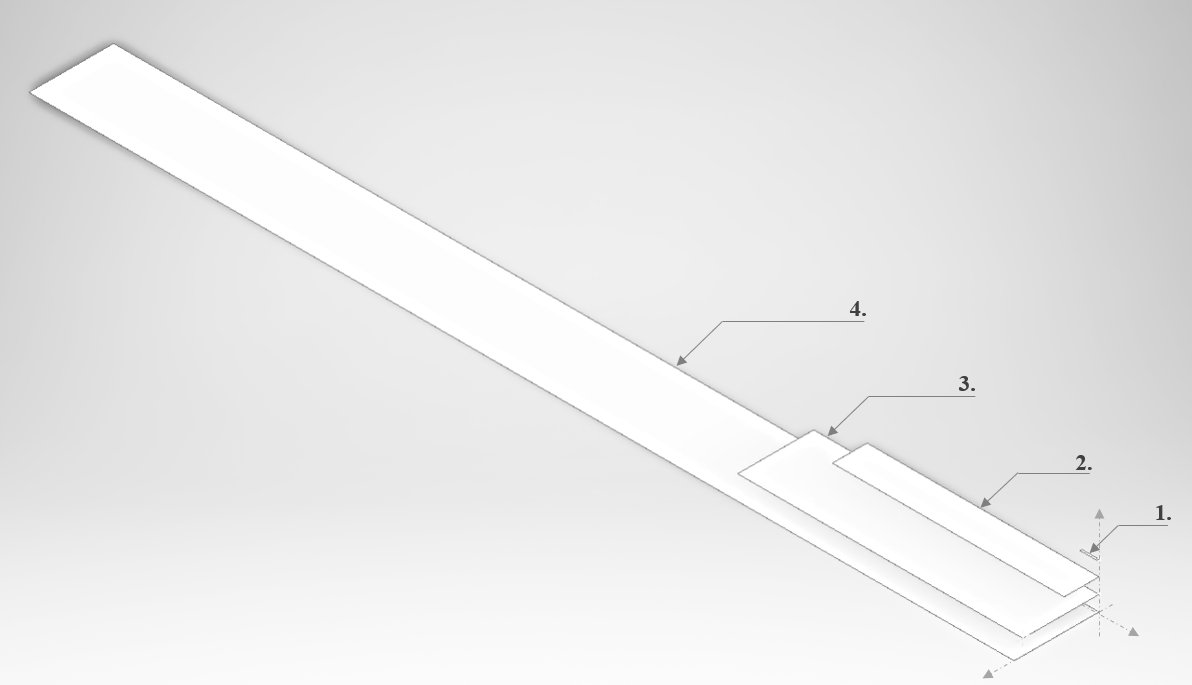
\includegraphics[width=\textwidth]{figures/iso-view.png}
    \caption{3D isotropic view of the comparison}
    \label{fig:3D-wings}
\end{figure}

%%%%%%%%%% Aim and Objectives %%%%%%%%%%
\section{Aim and Objectives}
\label{sec:aim+obj}
%\begin{itemize}
 %   \item Develop a computational method to study flutter and divergence behaviour.
 %   \item The aim is to use linear method for IXP to perform a preliminary parameter study.
 %   \item Develop into a nonlinear tool for FYP for a better study.
%\end{itemize}
\section*{Aims}
To develop a computational model to perform a parameter study on aeroelastic responses of aircraft wings with high aspect ratio.

\section*{Objectives} 
\begin{enumerate}
    \item Research existing experimental literature to use as a benchmark for the computational model that will be developed. 
    \item Explore literature on different numerical methods and decide on the most suitable model for the project. From these literature, 
    \item Investigate the existing MATLAB code for flutter calculation from the Introduction to Aeroelasticity and Loads by Jan Wright and Jonathan Cooper \cite{Wright2015INTRODUCTIONLOADS}.
   % \item Adapt the existing code to cater for a non-linear model. Based the model from numerical literature explored. Dimensions of aircraft already being investigated previously in experimental projects will be used in the model to validate the code.
   \item Create a MATLAB script based on the eigenvalue solution method to calculate flutter speed and divergence speed.
    \item Test the code against different existing results to validate the code.
    \item Upon obtaining results from different models, an analysis will be carried out on the effect of the chosen varied parameters and their effects on aeroelastic response of the models.
\end{enumerate}
\cleardoublepage
\newpage
%%%%%%%%%% Technical/Scientific Methodology %%%%%%%%%%
\section{Methodology}
\label{sec:method}
%\begin{itemize}
    %\item Computational and analytical method using \textbf{eigenvalue solutions} of the flutter equation.
    %\item From existing code
    %\item New one
    %\item Different models
    %\item Compare to existing experimental results
    %\item Benchmarking against the existing results
    %\item Use the code to analyse the aeroelastic behaviour of SUGAR High
%\end{itemize}
\subsection{Eigenvalue Solutions}
\label{sec:eig}
\iffalse
The method of determining the speed at which flutter occurs used in this study was the eigenvalue solutions. The inertia, structural and aerodynamic models used were explained in section \ref{sec:background}. The full aeroelastic equation was stated ealier as equation (6). Eigenvalues were obtained from this equation. 
\iffalse
The full aeroelastic equation can be simplified and represented as\\
\begin{equation}\label{eq:simplified-aeroe}
    mA\ddot{q}+\rho VB\dot{q}+\{\rho V^2 C+E\}q = 0
\end{equation}
\fi
The eigenvalues can be obtained by solving the determinant of the gathered 2x2 matrix of the full aeroelastic equation. This yields a quatic equation. Both of these equations can be found in the appendix in equation\\

To obtain the eigenvalues, Routh-Hurwitz stability analysis was applied to the quartic equation which yielded,

\begin{equation}
    b_4b_1^2-b_1b_2b_3+b_0b_3^2 = 0
\end{equation}

The lowest positive root with zero imaginary part represented the speed at which flutter occurs.
\fi
The method of determining the speed at which flutter occurs used in this study was the eigenvalue solutions. The inertia, structural and aerodynamic models used were explained in section \ref{sec:background}. The full aeroelastic equation was stated ealier as equation (3). Eigenvalues were obtained from this equation. The full aeroelastic equation can be simplified and represented as\\
\begin{equation}\label{eq:simplified-aeroe}
    mA\ddot{q}+\rho VB\dot{q}+\{\rho V^2 C+E\}q = 0
\end{equation}

The eigenvalues can be obtained by solving the determinant of the gathered 2x2 matrix of the full aeroelastic equation.\\

\begin{equation}
    \begin{gathered}
    \begin{vmatrix} A_{11}\lambda^2+B_{11}V\lambda+C_{11}V^2+E_{11} & A_{12}\lambda^2+B_{12}V\lambda+C_{12}V^2\\
    A_{21}\lambda^2+B_{21}V\lambda+C_{21}V^2&A_{21}\lambda^2+B_{22}V\lambda+C_{22}V^2+E_{22}\end{vmatrix}=0
    \end{gathered}
\end{equation}

The solution of this resulted in a quartic equation\\
\begin{equation}\label{eq:b_n}
    b_4\lambda^4+b_3\lambda^3+b_2\lambda^2+b_1\lambda+b_0 = 0
\end{equation}
where $b_n$, represented the constant for each term which also include the $V$ terms.\\

To obtain the eigenvalues, Routh-Hurwitz stability analysis was applied to the quartic equation which yielded,

\begin{equation}
    b_4b_1^2-b_1b_2b_3+b_0b_3^2 = 0
\end{equation}

The lowest positive root with zero imaginary part represented the speed at which flutter occurs.

\subsection{Code development}
The MATLAB script was developed based on the numerical model described in section \ref{sec:eig}. Symbolic MATLAB was used to solved the Routh-Hurwitz equation (eq.(11)). The \textit{syms} command was used to define $V$ and $\lambda$ as variables to be solved for and the eigenvalue solutions were calculated.        

\subsection{Parameter study}
Bending stiffness (EI) and torsional stiffness (GJ) were varied by $\pm$2.5\% increments up to 10\%. The percentage increment was used instead of adding a certain value to make the increase and decrease of the parameter value comparable between different models. The important parameters are listed in table \ref{tab:data}
\begin{table}[H]
    \centering
    \caption{Wing model parameters}
    \includestandalone{tables/parameters}
    \label{tab:data}
\end{table}

\subsection{Validation against existing studies}
Results from the calculations done using the model created were then being compared against the existing results to validate and test the limitations of the model.

%\textbf{VALIDATION}
%\textbf{ADD ERROR TABLE}
%\textbf{Do graph of this - obtained vs. reported results}
%\textbf{what's the limit, quatify the validity, limits}
%\textbf{what makes it works}
%\cleardoublepage

%%%%%%%%%% Preliminary Studies %%%%%%%%%%
\section{Preliminary Studies}
\label{sec:prelim}
This section presents the results from this study as well as the conclusion drawn from the analysis. The results from the MATLAB script were compared to the results from literature. The main parameters of these wings were listed in table \ref{tab:data}. Other relevant parameters can be found in table \ref{tab:TandD-exp-wing-data} and table \ref{tab:Goland-wing-data}. The error for each model was shown in table \ref{tab:error}. The average error was calculated to be 10.54\%; this was satisfactory for the preliminary study.
\vspace{-.5cm}
\begin{table}[H]
    \centering
    \caption{Benchmaking of results and their errors}
    \includestandalone{tables/error}
    \label{tab:error}
\end{table}

The baseline model from Wright and Cooper \cite{Wright2015INTRODUCTIONLOADS} (WC) exhibited the smallest error of less than 1\%. This was expected as the method was demonstrated to be suitable for this wing in the literature. Other errors showed a trend of increasing with the increase in aspect ratio with the highest error percentage seen in the SUGAR High model - 16.84\%.\\
%\textbf{WHY ARE YOU DOING IT}

\iffalse
\begin{figure}[H]
    \centering
    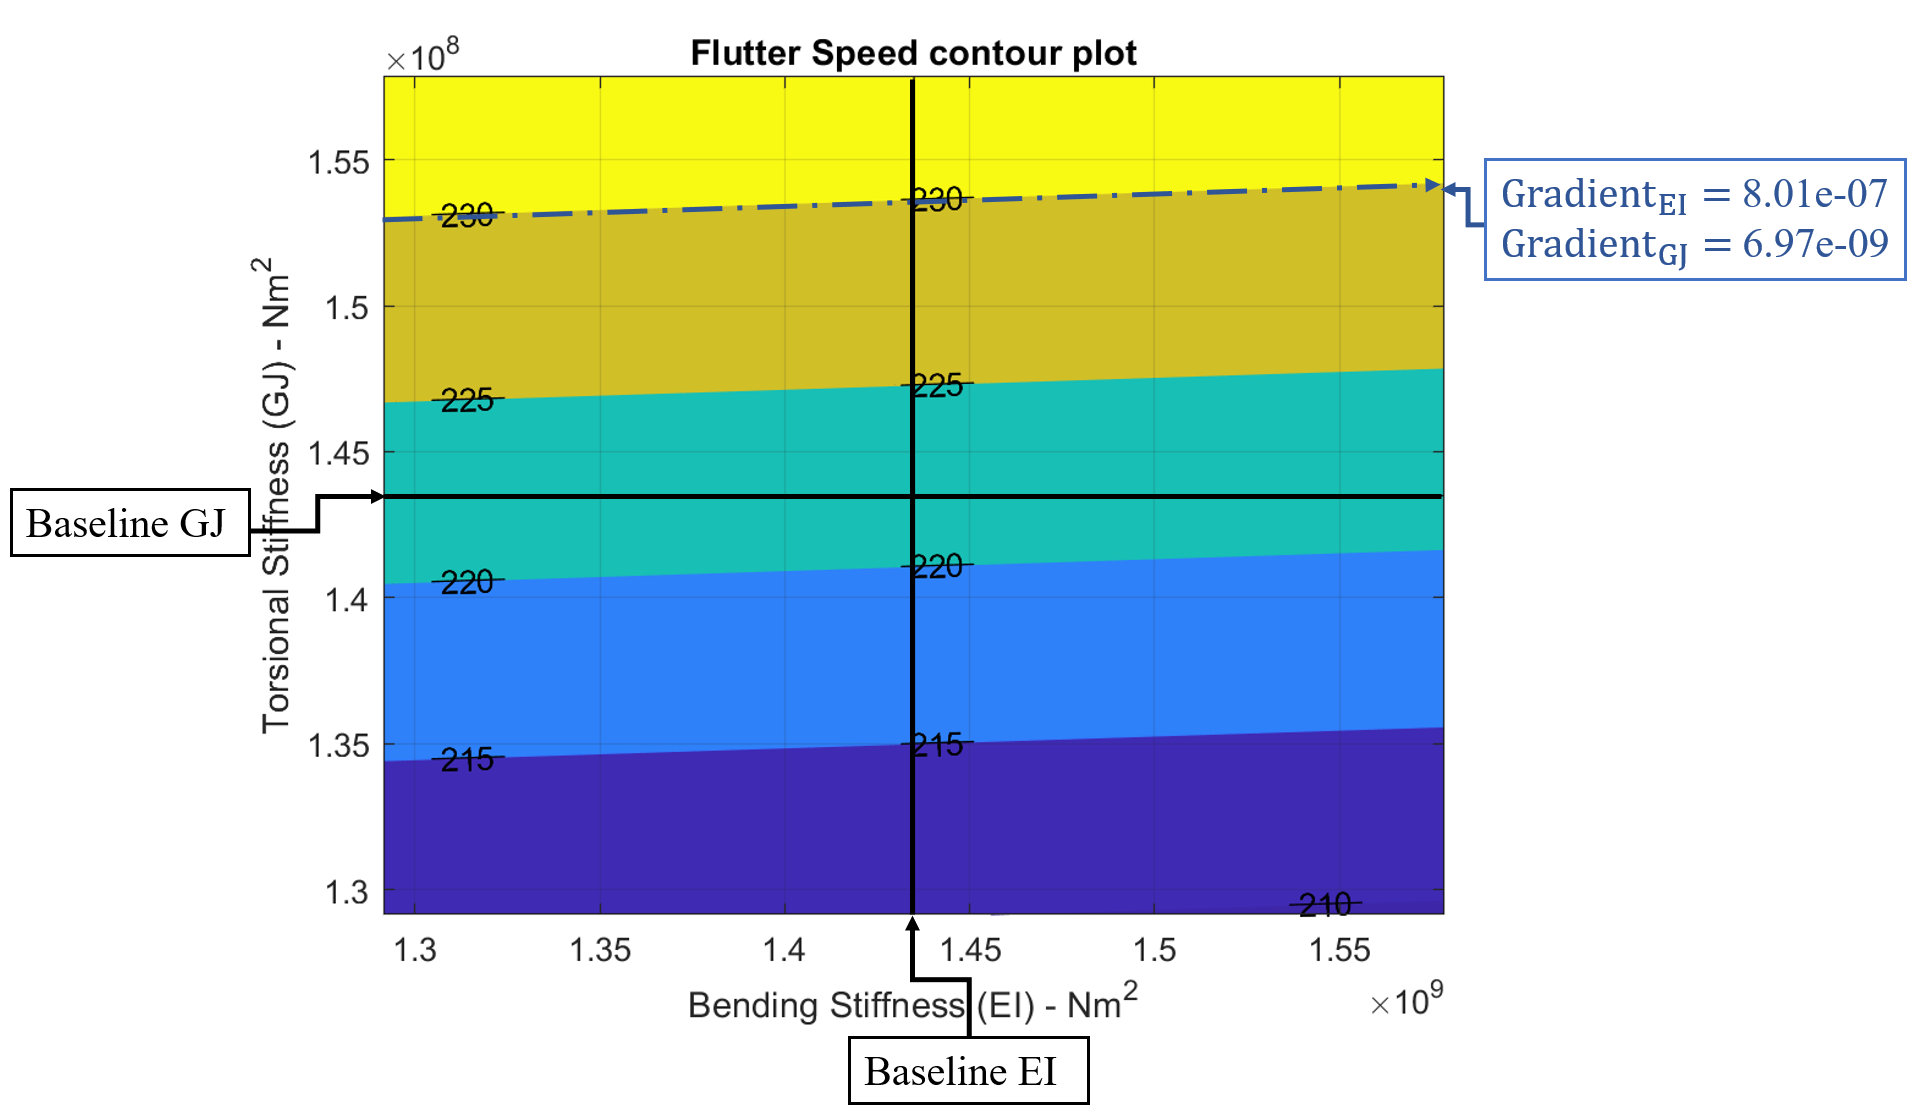
\includegraphics[width = \textwidth]{figures/SUGAR_flutt.png}
    \caption{Flutter speed plot for the SUGAR High conceptual wing}
    \label{fig:SUGAR-flutt}
\end{figure}

\begin{figure}[H]
    \centering
    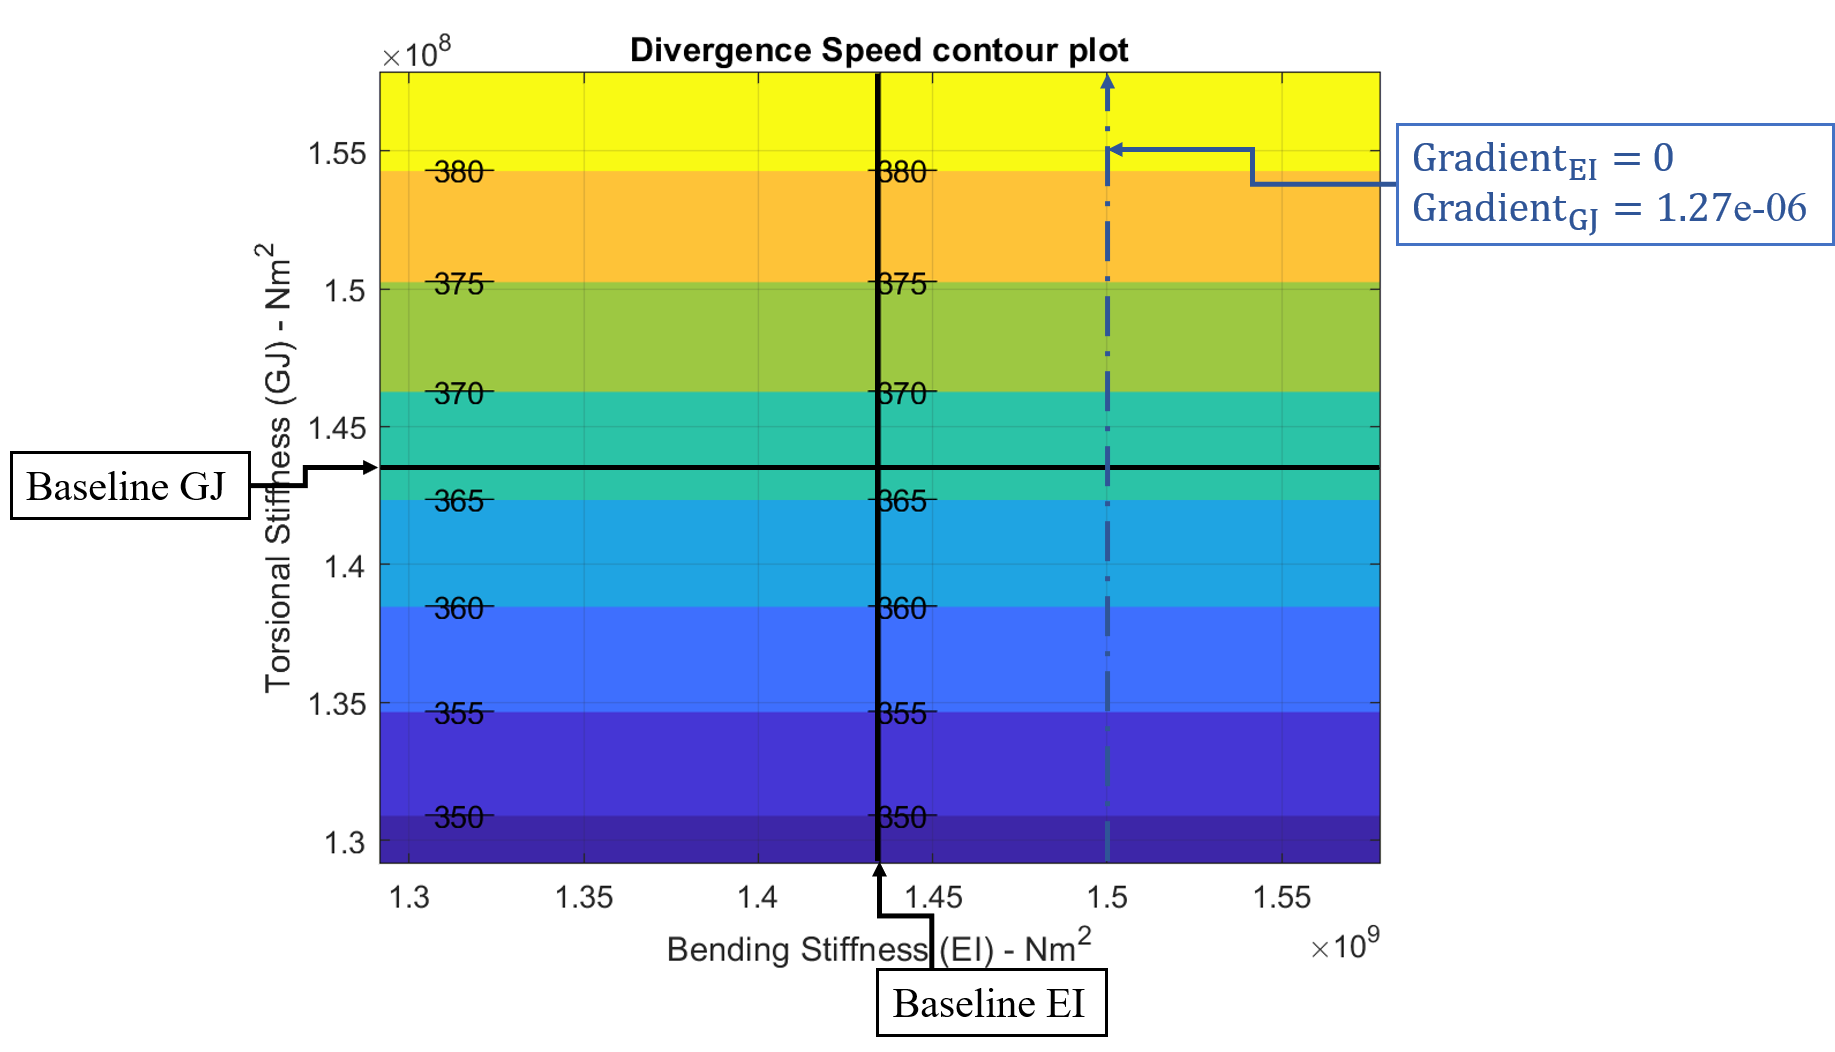
\includegraphics[width = \textwidth]{figures/SUGAR_div.png}
    \caption{Divergence speed plot for the SUGAR High conceptual wing}
    \label{fig:SUGAR-div}
\end{figure}
\fi
%\iffalse
\vspace{-.5cm}
\begin{figure}[!hbt]
    \begin{minipage}{.5\textwidth}
    \centering
    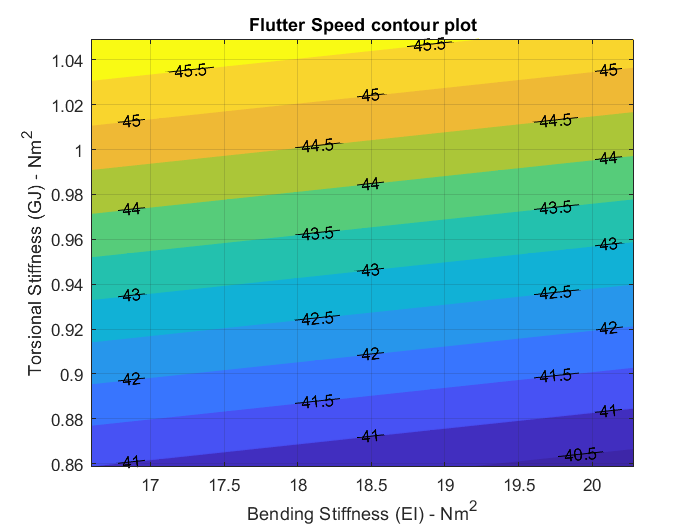
\includegraphics[width = \textwidth]{figures/flutter.png}
    \caption{SUGAR High flutter plot}
    \label{fig:SUGAR-flutt}
    \end{minipage}%
    \begin{minipage}{.5\textwidth}
    \centering
    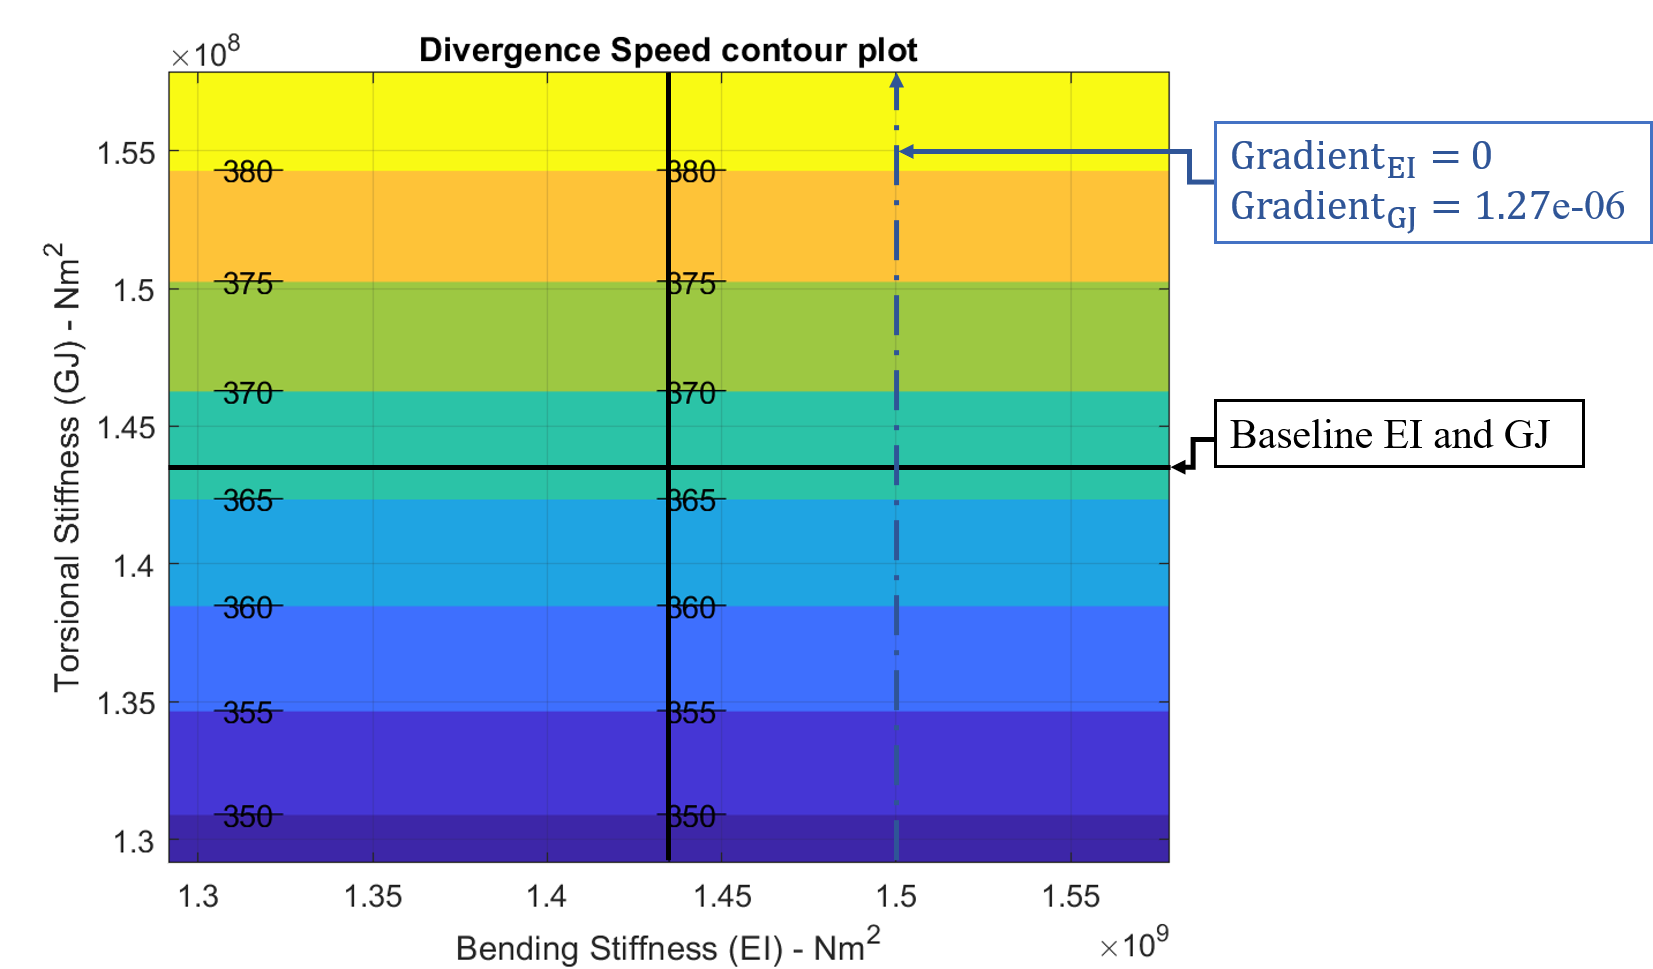
\includegraphics[width = \textwidth]{figures/divergence.png}
    \caption{SUGAR High divergence plot}
    \label{fig:SUGAR-div}
    \end{minipage}
\end{figure}
%\fi
%\textbf{TRENDS}

%\begin{itemize}
%    \item Reasons for discrepancies - nonlinearity
%\end{itemize}
The result of the analysis of the flutter and divergence behaviour of NASA's SUGAR High with the parameter of EI and GJ varied are illustrated below. The flutter behaviour is shown in figure \ref{fig:SUGAR-flutt} and the divergence behaviour is shown in figure \ref{fig:SUGAR-div}.\\
\vspace{-1cm}
\begin{wrapfigure}[18]{l}{9cm}
    \centering
    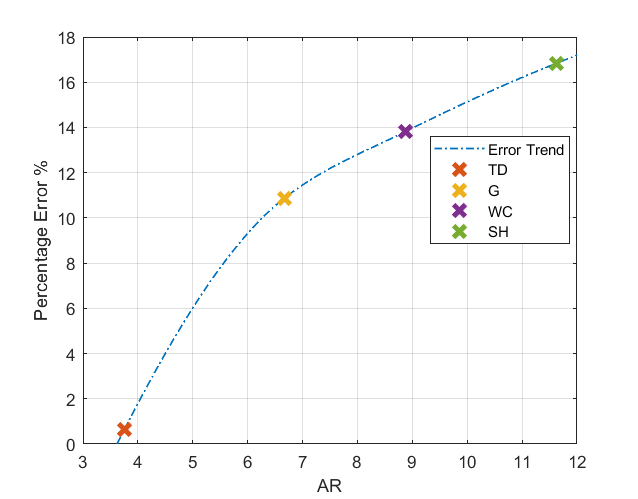
\includegraphics[width = 9cm]{figures/error-trend.png}
    \caption{Relationship of aspect ratio and the discrepancies of the results calculated.}
    \label{fig:error}
\end{wrapfigure}
\\ \\
Figure \ref{fig:error} shows the error trend proposed as observed by comparing the results calculated from the model developed against the existing analytical results. These errors were shown individually for each model in table \ref{tab:error}. The discrepancies was concluded to be a result of nonlinearities which were not included in this model as the error from the computational model increases with respect to the increase in aspect ratio. This is because an increase in aspect ratio decreases the rigidity of the wing. Large wing tip deflection leads to aerodynamic forces acting not vertically to the wing.\\ \\ \\

The blue dashed line in figure \ref{fig:error} shows the error trend of the computational model. It can be seen that the trend increases with aspect ratio but the rate of increase decreases as the aspect ratio get higher. With this trend, the error might be limited at around 20\%. However, the model can be improved with the inclusion of nonlinearities to mitigate this discrepancies.

\subsection{Initial Conclusions}
\iffalse
\begin{itemize}
    \item Flutter is affected by both
    \item Divergence is only affected by Torsional Stiffness
    \item How to increase EI
    \begin{itemize}
        \item Material used - stiffer materials - affects E
        \item Add strut - affects I
    \end{itemize}
    \item How to increase GJ
    \begin{itemize}
        \item sweep back - decrease torsion
    \end{itemize}
    \item It can be seen in figure \ref{fig:SUGAR-flutt} that changes in bending stiffness (EI) has a greater impact to the flutter behaviour than the torsional stiffness (GJ). On the other hand, only GJ affects the divergence behaviour (figure \ref{fig:SUGAR-div}). This can be concluded as a result of how flutter depends on oscillations but divergence does not.\\
\end{itemize}
\fi
It can be seen in figure \ref{fig:SUGAR-flutt} that changes in bending stiffness (EI) has a greater impact to the flutter behaviour than the torsional stiffness (GJ). On the other hand, only GJ affects the divergence behaviour (figure \ref{fig:SUGAR-div}). This can be concluded as a result of how flutter depends on oscillations but divergence does not. Therefore, to delay the onset of flutter, increasing EI can achieve this, while increasing GJ delays divergence. EI can be increased to opting for a stiffer material or adding strut to the wing configuration. GJ can be increased by sweeping back the wing. This decreases torsion on the wing.

%%%%%%%%%% Initial Conclusions and Risk Management %%%%%%%%%%
\section{Risk Management}
\label{sec:risk}
%Risk of model not working
%not getting parameter
%valiadste model again multiple case to make sure it works
This project used a combination of computational and numerical methods. The risk in this study included the risk of not being able to produce a working MATLAB script. This risk was mitigated by using an existing MATLAB script \cite{Wright2015INTRODUCTIONLOADS} for flutter speed calculation as a starting point as this means that there was a backup script that can be modified to take in ranges of different parameters for calculation, in the case that a new script cannot be made to yield a satisfactory result.\\

Moreover, one of the difficulties encountered in this project was obtaining information for parameters. This was found to be a bigger challenge than expected as many studies do not document every parameters used in the models. Another risk was that a number of researches were done using imperial based unit and to make the results comparable, parameters need to be converted into SI units correctly. This risk was mitigated by rechecking the conversion to make sure there were no errors.

%%%%%%%%%% Future Work %%%%%%%%%%
\section{Future Work}
\label{sec:future-work}
\iffalse
\begin{itemize}
    \item other parameters
    \item nonlinear
\end{itemize}
The model developed in this study containes many linear assumption which simplified the model for the preliminary studies.
\begin{enumerate}
    \item Structure model assumed no coupling between the bending and torsion mode.
    \item Only one assumed more shape was included for bending and torsion.
    \item Aerodynamic force was assumed to act vertically to the lifting surface which is not the case in most high AR wing.
    \item Limit cycle oscillation was not included in the study.
\end{enumerate}
\fi
The errors and limitations in this model was mentioned in section \ref{sec:prelim}. This suggested a modification to a higher fidelity and a more complex model to be developed for future work. This includes the inclusion of nonlinearities, the inclusion of finite difference method, computational fluid dynamic analysis and a nonlinear finite element analysis. Existing toolbox such as UM/NAST and ONERO stall model can also be investigated. This method only assumed 2 mode shapes, more mode shapes can be included for a better analysis.\\

Furthermore, other ranges of parameters such as mass per unit and second moment of area can be varied for parameter study of other properties. Another important aeroelastic behaviour - limit cycle oscillation should also be looked at in future works with the inclusion of nonlinearities as this behaviour is useful when occurs before flutter; it helps limit the fatality of flutter and limit the occurance of divergence.

%%%%%%%%%% Project Work plan %%%%%%%%%%
\section{Work Plan}
\begin{figure}[H]
    \centering
    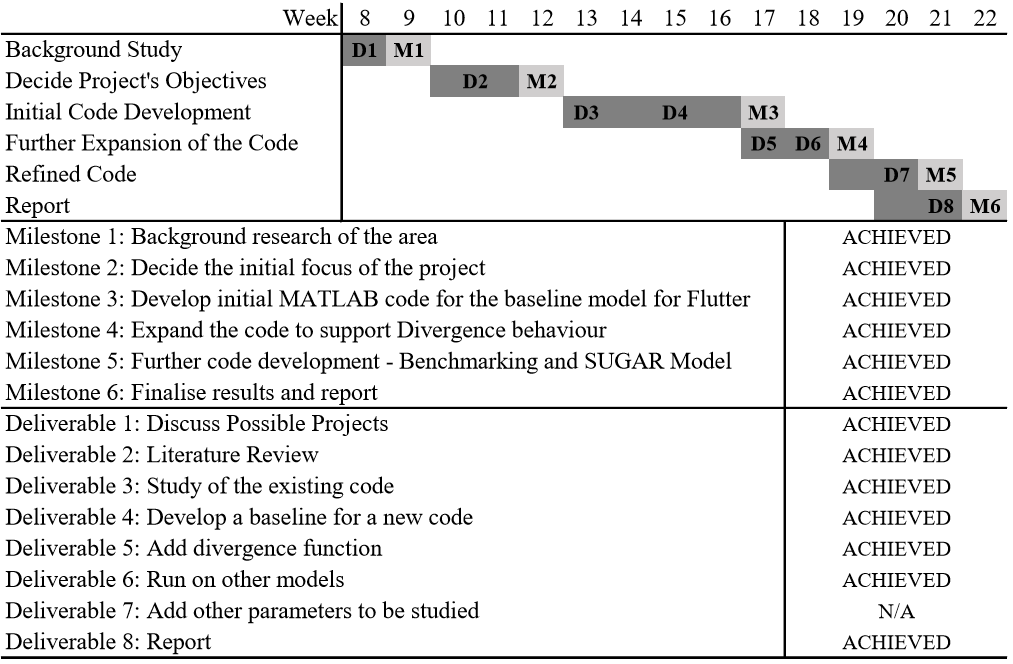
\includegraphics[width = .9\textwidth]{figures/dandm.png}
    %\label{fig:my_label}
\end{figure}

\textbf{Final Year Research Project}
\begin{figure}[H]
    \centering
    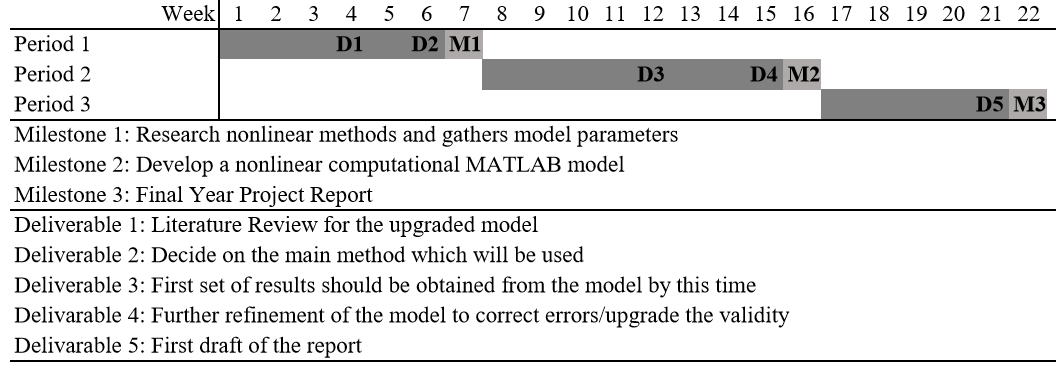
\includegraphics[width = .9\textwidth]{figures/fyp.png}
    %\caption{Caption}
    %\label{fig:my_label}
\end{figure}

\cleardoublepage

%%%%%%%%%% Reference %%%%%%%%%%
\newpage
\bibliography{references.bib}
\cleardoublepage
\pagenumbering{roman} 
%%%%%%%%%% Appendices %%%%%%%%%%
\section*{Appendix}
\appendix
\appendixname{ A}
\label{app:2D-para}
\begin{figure}[H]
    \centering
    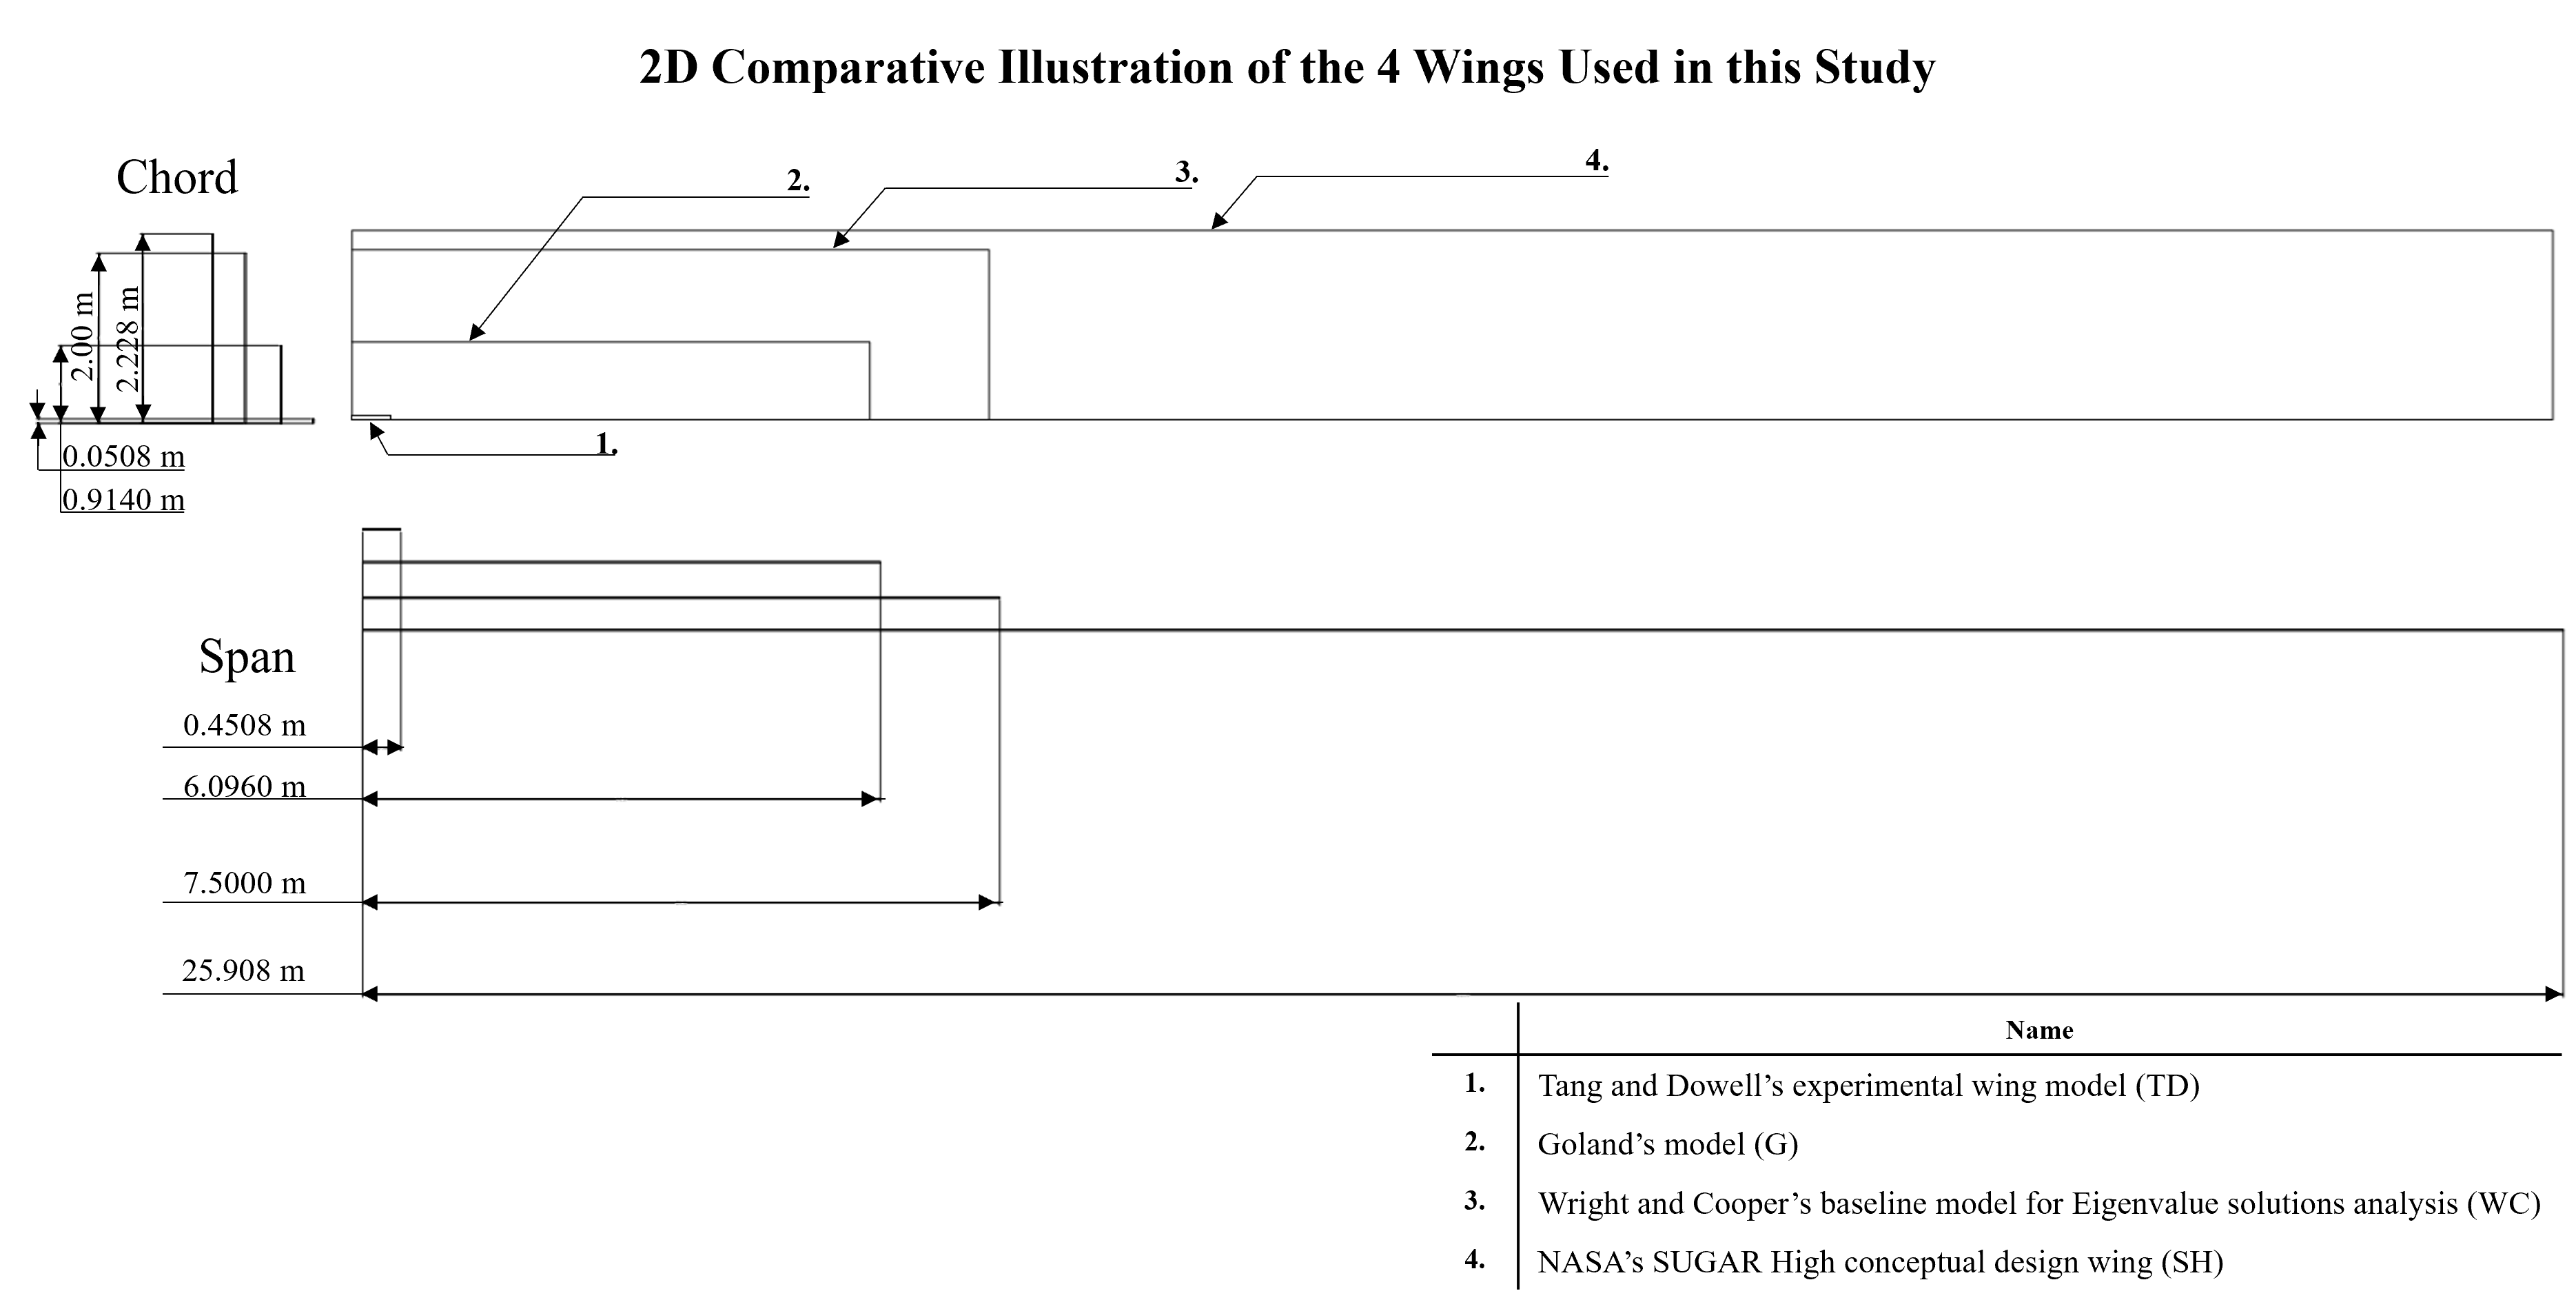
\includegraphics[width =\textwidth]{figures/para.png}
    \caption{2D Illustration of the models}
    \label{fig:2D-wings}
\end{figure}
\iffalse
\appendixname{ B}
Determinant of the gathered aeroelastic equation
\begin{equation}\label{eq:determinant}
    \begin{gathered}
    \begin{vmatrix} A_{11}\lambda^2+B_{11}V\lambda+C_{11}V^2+E_{11} & A_{12}\lambda^2+B_{12}V\lambda+C_{12}V^2\\
    A_{21}\lambda^2+B_{21}V\lambda+C_{21}V^2&A_{21}\lambda^2+B_{22}V\lambda+C_{22}V^2+E_{22}\end{vmatrix}=0
    \end{gathered}
\end{equation}

\begin{equation}\label{eq:b_n}
    b_4\lambda^4+b_3\lambda^3+b_2\lambda^2+b_1\lambda+b_0 = 0
\end{equation}
where $b_n$, represented the constant for each term which also include the $V$ terms.
\fi
%\cleardoublepage
%\newpage
%\appendixname{ C}
\label{app:other-para}
\begin{table}[H]
    \centering
    \caption{Tang and Dowell Experimental wing model\cite{Tang2001ExperimentalWings} and Goland's model \cite{CHETANNICHKAWDE2006NONLINEARCONTINUATION} data}
    \includestandalone{tables/TDandG}
    \label{tab:TandD-exp-wing-data}
\end{table}
\begin{table}[H]
    \centering
    \caption{Wright and Cooper \cite{Wright2015INTRODUCTIONLOADS} baseline model and SUGAR High wing model \cite{Bradley2015SubsonicExploration} data}
    \includestandalone{tables/WCandSH}
    \label{tab:Goland-wing-data}
\end{table}
\cleardoublepage
\newpage
\appendixname{ C}
\label{app:ei-gj}
\begin{table}[H]
    \centering
    \caption{EI and GJ parameter increments}
    \includestandalone{tables/EIGJ}
    \label{tab:ei-gj}
\end{table}
%\cleardoublepage
%\newpage
\appendixname{ D}
\label{app:other-wings}
\begin{figure}[!hbt]
    \begin{minipage}{.5\textwidth}
    \centering
    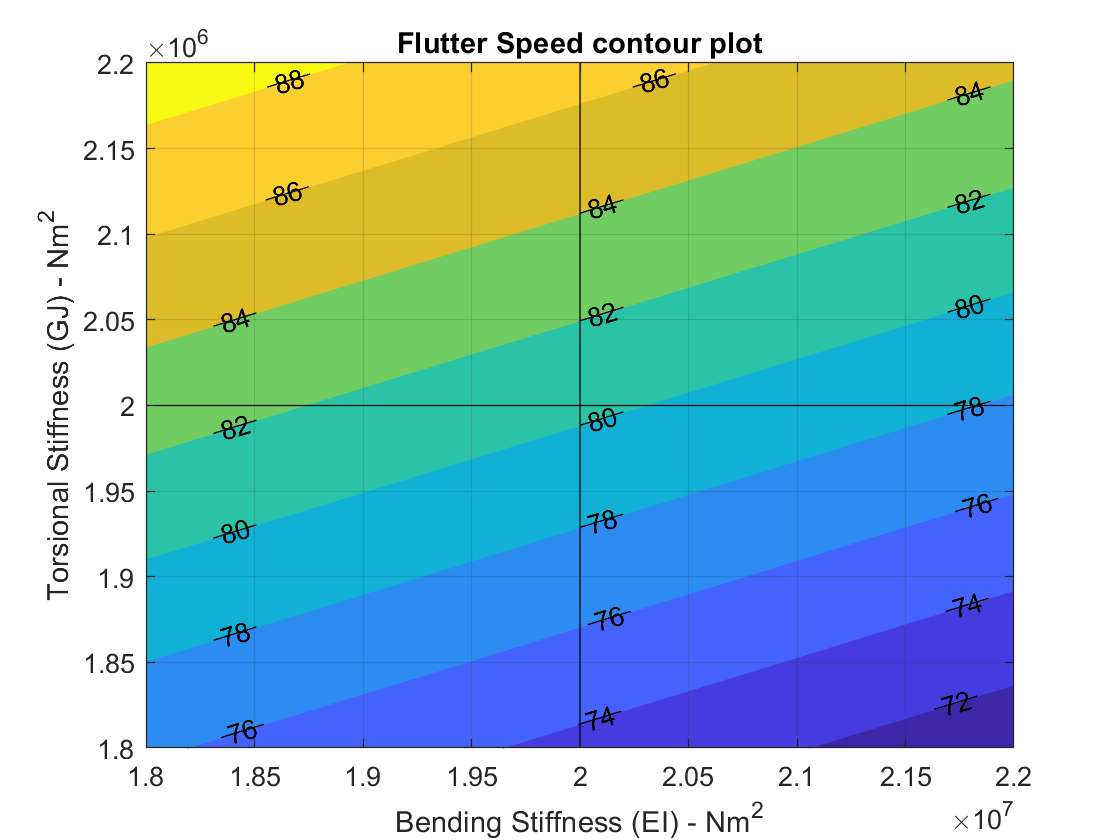
\includegraphics[width = \textwidth]{figures/Cooper_flutter.png}
    \caption{Baseline model flutter calculation}
    \label{fig:JandJ-flutter}
    \end{minipage}%
    \begin{minipage}{.5\textwidth}
    \centering
    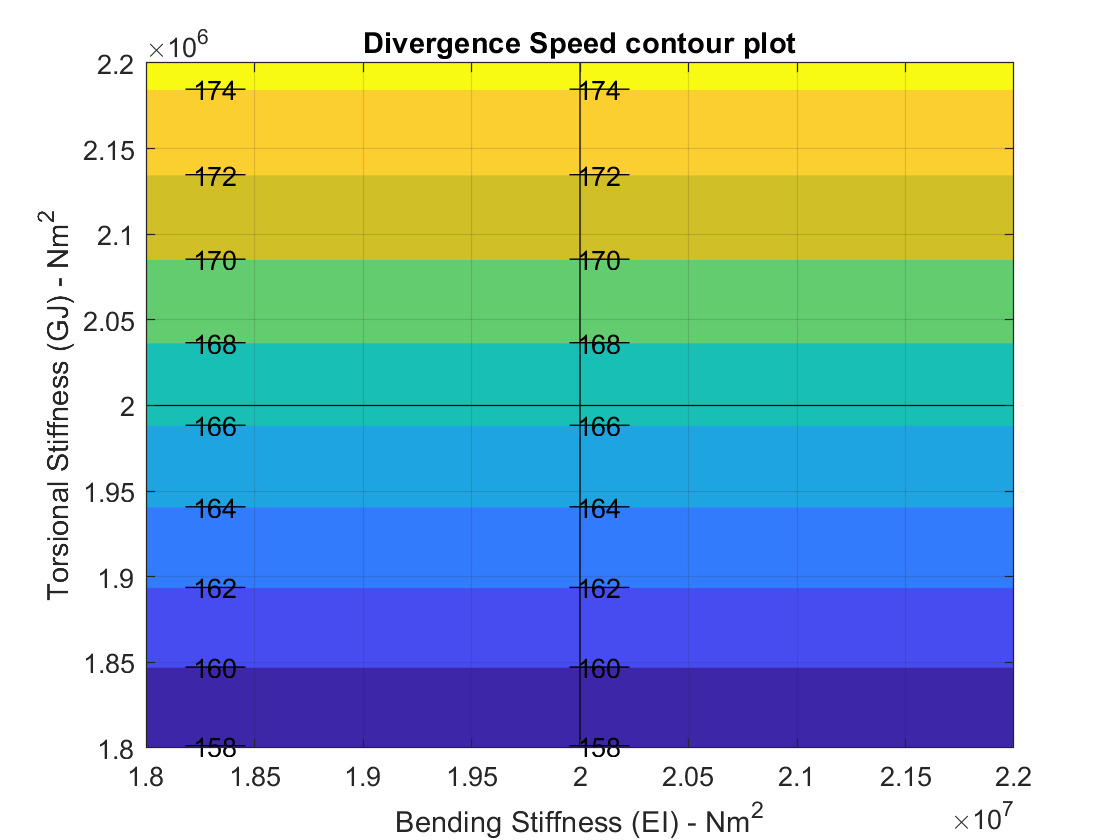
\includegraphics[width = \textwidth]{figures/Cooper_divergence.png}
    \caption{Baseline model divergence calculation}
    \label{fig:JandJ-div}
    \end{minipage}
\end{figure}
\begin{figure}[!hbt]
    \begin{minipage}{.5\textwidth}
    \centering
    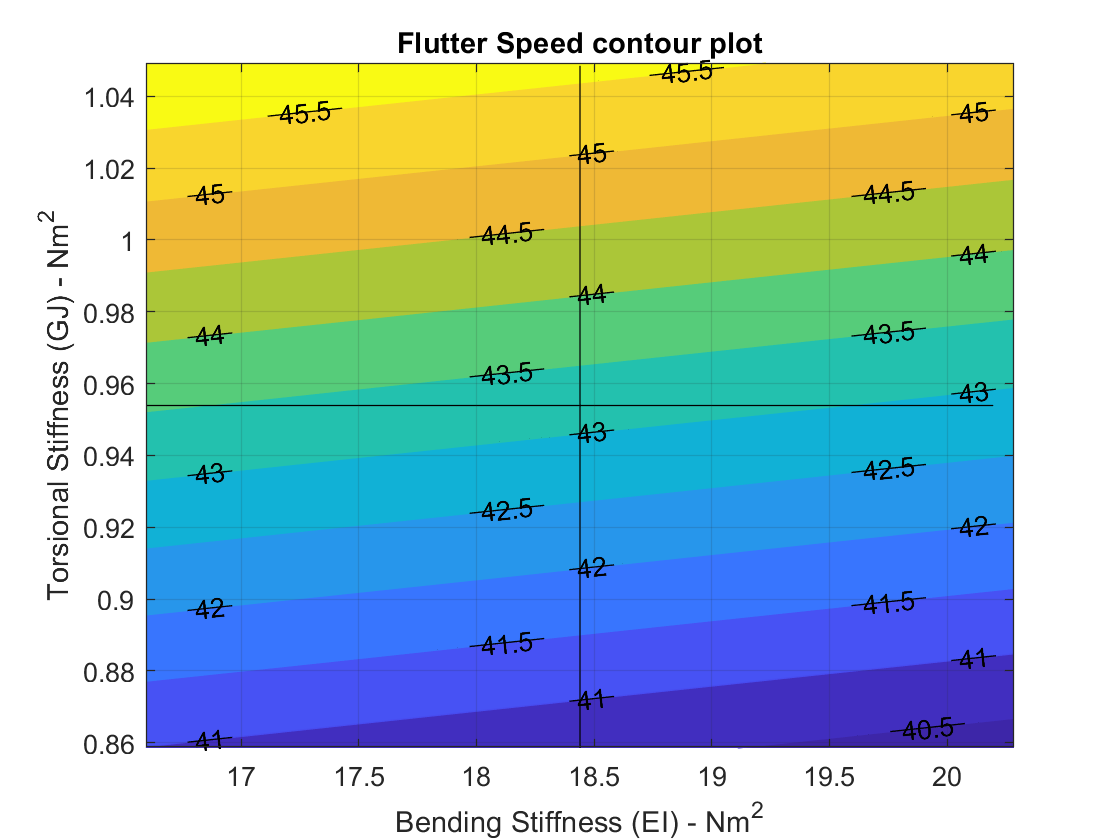
\includegraphics[width = \textwidth]{figures/Tang_flutter.png}
    \caption{Tang and Dowell flutter calculation}
    \label{fig:TandD-flutter}
    \end{minipage}%
    \begin{minipage}{.5\textwidth}
    \centering
    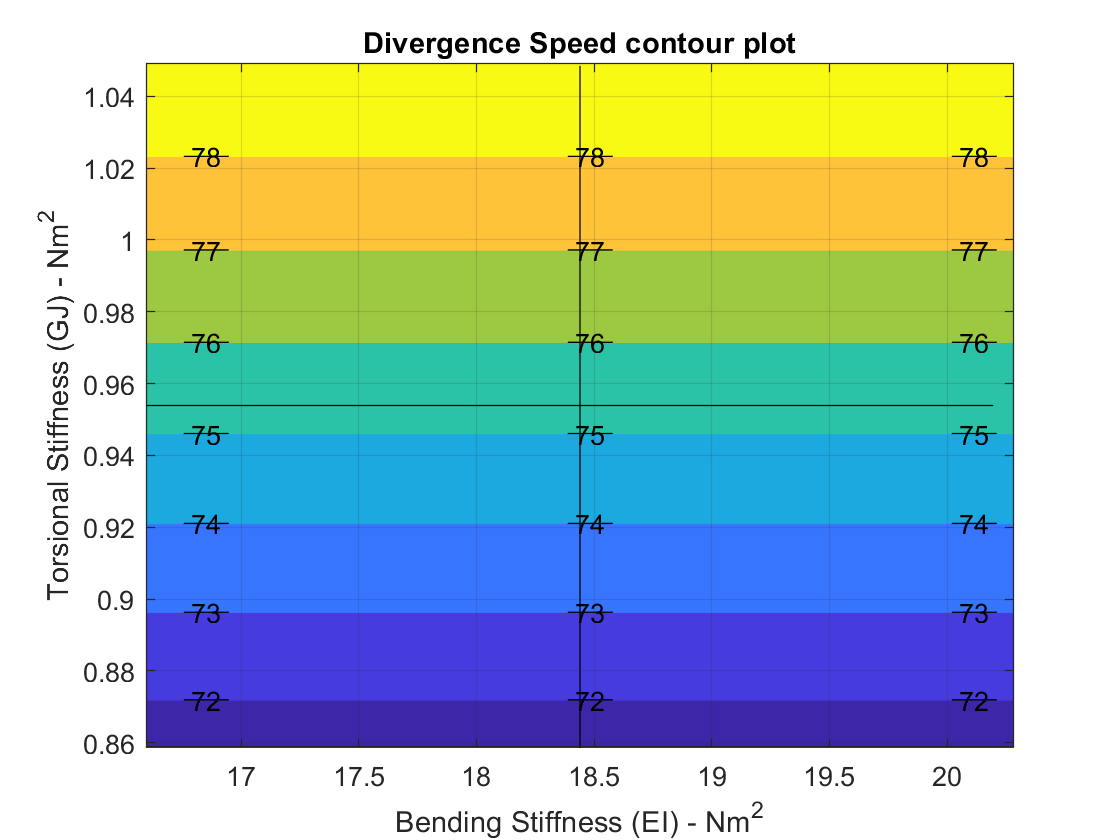
\includegraphics[width = \textwidth]{figures/Tang_divergence.png}
    \caption{Tang and Dowell divergence calculation}
    \label{fig:TandD-div}
    \end{minipage}
\end{figure}
\begin{figure}[H]
    \begin{minipage}{.5\textwidth}
    \centering
    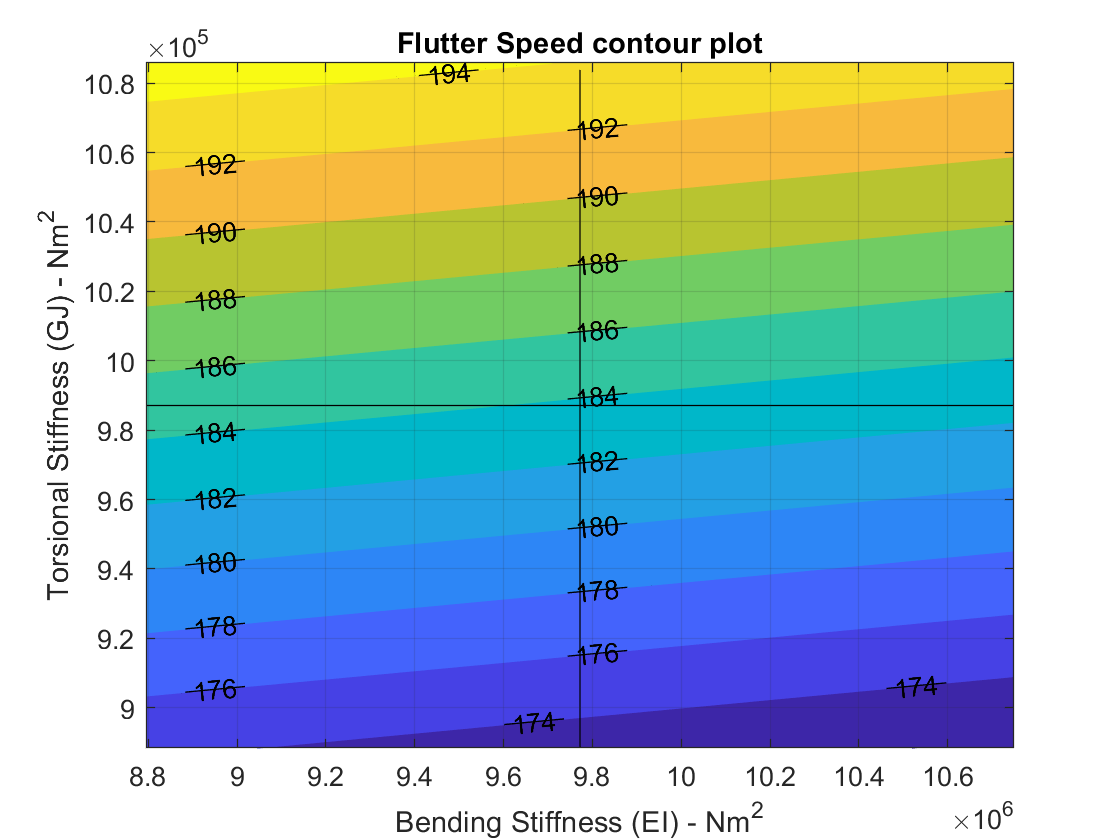
\includegraphics[width = \textwidth]{figures/Goland_flutter.png}
    \caption{Goland heavy wing flutter calculation}
    \label{fig:Goland-flutter}
    \end{minipage}%
    \begin{minipage}{.5\textwidth}
    \centering
    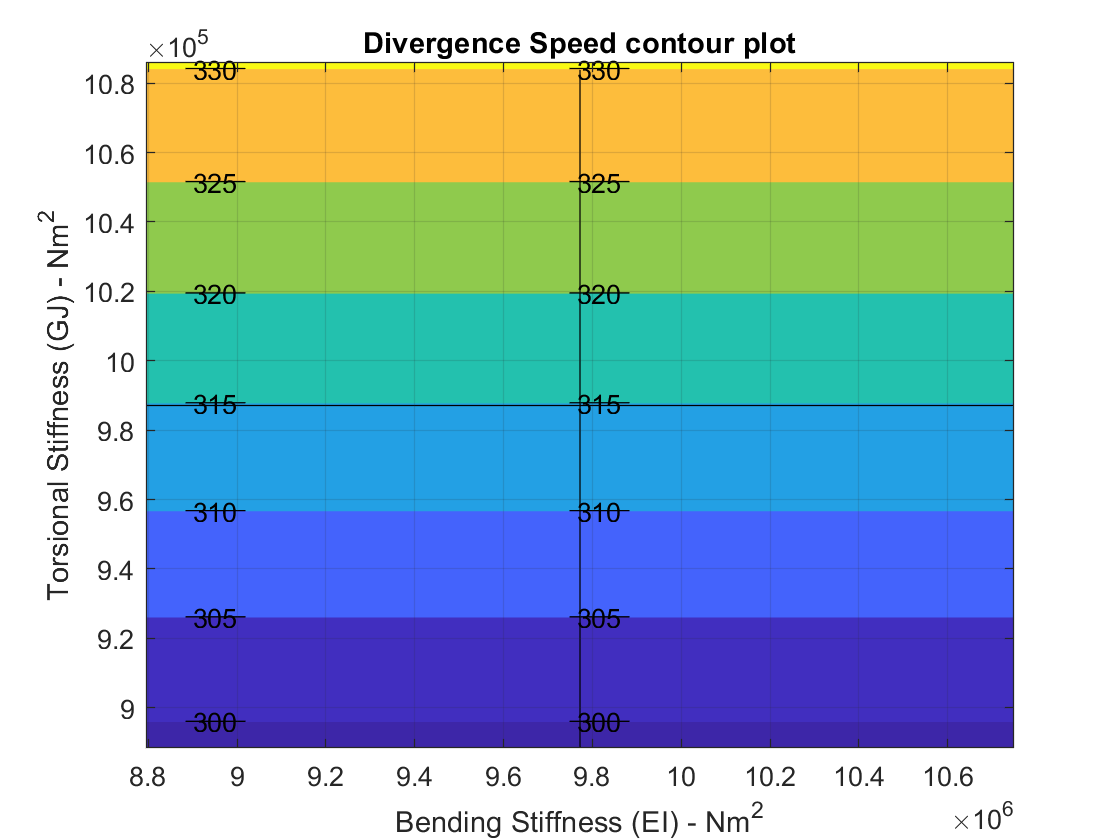
\includegraphics[width = \textwidth]{figures/Goland_divergence.png}
    \caption{Goland heavy wing divergence calculation}
    \label{fig:Goland-div}
    \end{minipage}
\end{figure}

\end{document}
